\capitulo{5}{Aspectos relevantes del desarrollo del proyecto}

\section{Herramientas de control de tareas: Kanban y Scrum}

Para llevar un control efectivo de las tareas y asegurar la evolución continua del proyecto, se han utilizado metodologías ágiles como \textbf{Kanban} y \textbf{Scrum}.

\begin{itemize}
    \item \textbf{Kanban:} Se utilizó Kanban debido a su flexibilidad y enfoque visual. Kanban nos permitió gestionar el flujo de trabajo mediante tarjetas en un tablero visual, donde las tareas se movían de una columna a otra (de "Por hacer" a "En progreso" y "Hecho"). Esto facilitó una vista clara de las tareas pendientes, así como una priorización y reestructuración rápida de las mismas según los requerimientos que surgían.
    
    \item \textbf{Scrum:} Se implementó Scrum en ciclos de trabajo denominados \textit{sprints}, con duraciones de dos semanas. Cada \textit{sprint} comenzaba con una reunión en la que se revisaban en retrospectiva las tareas realizadas el último \textit{sprint} y se planificaban los objetivos y metas para la siguiente reunión. Este ciclo permitió adaptar las prioridades en función de los avances realizados y los desafíos encontrados, proporcionando un proceso estructurado que se ajustó bien a las necesidades de fases más avanzadas del desarrollo.
\end{itemize}

El uso combinado de ambas metodologías facilitó tanto la flexibilidad como la estructura necesarias en diferentes fases del proyecto, contribuyendo a un flujo de trabajo eficiente y orientado a resultados.

\section{Formación y aprendizaje necesario}

El desarrollo del proyecto requirió adquirir nuevos conocimientos y profundizar en diversas tecnologías y técnicas de análisis. A continuación, se describe la formación llevada a cabo en las herramientas y algoritmos más relevantes.

\subsection{Estudio del algoritmo TRACLUS}

El enfoque principal de este proyecto ha sido estudiar en profundidad el algoritmo \textbf{TRACLUS}, destinando una gran parte de las horas de investigación a comprender su funcionamiento y potencial para el análisis de trayectorias. Este algoritmo se basa en la segmentación y agrupación de trayectorias, permitiendo identificar sub-trayectorias comunes dentro de un conjunto de datos. Esto lo convierte en una herramienta valiosa para descubrir patrones significativos en datos de trayectorias. La investigación incluyó la revisión de artículos académicos y la exploración de cómo ajustar los parámetros de TRACLUS para maximizar su efectividad en el contexto específico del proyecto.

Adicionalmente, se evaluó el uso de una implementación de TRACLUS disponible en una biblioteca externa, explorando su viabilidad y características. Aunque esta versión fue útil para los primeros experimentos, se consideraron también posibles variantes y adaptaciones del algoritmo, con el fin de entender mejor el alcance y la adaptabilidad de TRACLUS.

\subsubsection{Propuesta de variantes de TRACLUS}

Durante el desarrollo del proyecto, se analizaron varias propuestas de variantes del algoritmo TRACLUS que han surgido en estudios recientes. Aunque finalmente no se utilizaron, la investigación detallada de estos derivados fue enriquecedora y ayudó a contrastar enfoques para una implementación eficiente. Las variantes de TRACLUS estudiadas fueron:

\begin{itemize}
    \item \textbf{GTraclus:} Una variante diseñada para ejecutarse en unidades de procesamiento gráfico (GPU), optimizando la eficiencia del algoritmo al aprovechar la capacidad de procesamiento paralelo de las GPUs \cite{gtraclus}.

    \item \textbf{ST-TRACLUS:} Esta versión incorpora una dimensión temporal además de la espacial, permitiendo realizar agrupamientos espaciotemporales de trayectorias, lo cual mejora la calidad del análisis para datos donde el tiempo es una variable relevante \cite{st-traclus}.

    \item \textbf{ND-TRACLUS:} Una extensión de TRACLUS que permite realizar el clustering en espacios de n dimensiones, expandiendo su aplicabilidad a trayectorias de mayor dimensionalidad \cite{nd-traclus}.

    \item \textbf{Neighborhood-Based Trajectory Clustering:} Una alternativa basada en densidad local de vecindad en lugar de densidad global. Este enfoque busca mantener la eficiencia de TRACLUS mientras reduce la necesidad de múltiples parámetros de entrada.

    \item \textbf{Adaptive Trajectory Clustering based on Grid and Density (ATCGD):} Un método que introduce una cuadrícula y criterios de densidad para el análisis de patrones móviles, buscando reducir la complejidad computacional y la carga de trabajo en la calibración de parámetros, especialmente en aplicaciones a gran escala como la de trayectorias de vehículos en sistemas de transporte inteligente \cite{atcgd}.
\end{itemize}


\subsubsection{Técnicas de clustering complementarias}

Paralelamente a la investigación de las variantes de TRACLUS, se estudiaron técnicas adicionales de clustering, dado que el algoritmo requiere la clusterización de segmentos para su evaluación final. Con el objetivo de evaluar la viabilidad y robustez de TRACLUS, se analizaron diversas técnicas de clustering, y tras descartar varias por inviabilidad, se optó finalmente por implementar las siguientes metodologías de \texttt{scikit-learn}:

\begin{itemize}
    \item \textbf{DBSCAN:} Algoritmo basado en densidad que identifica clusters de alta densidad separados por regiones de menor densidad, adecuado para datos espaciales y resistente al ruido.
    
    \item \textbf{OPTICS:} Similar a DBSCAN, pero permite una sensibilidad ajustable a la densidad, lo que lo hace más flexible para analizar datos con densidades variadas.

    \item \textbf{HDBSCAN:} Variante jerárquica de DBSCAN que ajusta automáticamente los parámetros de densidad, simplificando su aplicación en datos de densidad variable.

    \item \textbf{Spectral Clustering:} Algoritmo basado en el análisis de valores propios que es particularmente útil en datos no lineales o con clusters de formas complejas.

    \item \textbf{Agglomerative Clustering:} Método jerárquico ascendente que agrupa iterativamente elementos basándose en la proximidad, resultando útil en análisis donde la estructura jerárquica es relevante.
\end{itemize}

Cada técnica fue investigada en términos de sus características, sensibilidad a la densidad, capacidad de manejar ruido y aplicabilidad a datos espaciales. La exploración de estas técnicas permitió seleccionar aquellas que mejor se adaptaran a las necesidades específicas del proyecto y que complementaran el uso de TRACLUS en el análisis de trayectorias.


\subsection{Tiempos de Ejecución}    

El que podríamos considerar como el segundo punto más relevante, y sin duda uno de los aspectos críticos del proyecto, han sido los tiempos de ejecución. Debido a las grandes cantidades de datos a procesar, cada cálculo y visualización requerían una considerable cantidad de tiempo, por lo que la optimización de tiempos se convirtió en una prioridad clave para asegurar la viabilidad del proyecto.

\subsubsection{Visualización y Dibujado de Mapas}

Uno de los mayores desafíos de rendimiento fue la visualización de mapas, especialmente al intentar realizar representaciones detalladas y visualmente atractivas. Al analizar distintas bibliotecas de Python para dibujar y visualizar mapas, se probaron y compararon múltiples opciones combinadas entre si, como \texttt{pandas}, \texttt{geopandas}, \texttt{folium}, \texttt{folium.plugins}, \texttt{matplotlib.pyplot}, \texttt{matplotlib.colors}, \texttt{contextily}, \texttt{pyproj}, \texttt{seaborn}, \texttt{pydeck}, \texttt{shapely.geometry}, \texttt{sklearn.preprocessing} y \texttt{scipy.stats}.

Tras diversas pruebas de rendimiento y calidad visual, se optó por utilizar principalmente \texttt{contextily} y \texttt{matplotlib.pyplot} para la visualización de mapas, ya que estas bibliotecas ofrecieron la mejor relación entre rendimiento y calidad gráfica. Para la visualización de \textit{heatmaps}, se incluyeron \texttt{numpy} como las opciones más eficientes para generar mapas de calor. Sin embargo, para lograr un equilibrio óptimo entre rendimiento y visualización, se sacrificaron ciertas funcionalidades como el zoom en mapas interactivos y detalles visuales avanzados.

\subsubsection{Optimización del Algoritmo TRACLUS}

El algoritmo TRACLUS, por su complejidad, resultó ser la partes más lentas del sistema. Para abordar este desafío, se llevó a cabo un exhaustivo estudio de rendimiento, en el cual se identificaron las partes del código que consumían más recursos y tiempo de ejecución.

Como resultado de este análisis, se investigó la posibilidad de aplicar técnicas de paralelización y \texttt{threading} para mejorar la eficiencia del procesamiento. Sin embargo, la naturaleza del algoritmo, en combinación con el volumen de datos, limitó la efectividad de estas técnicas en algunas secciones críticas. A pesar de ello, ciertos aspectos del procesamiento pudieron ser paralelizados para aprovechar mejor los recursos de hardware, logrando una mejora en el tiempo total de ejecución.

\subsection{Librerías}

\begin{itemize}
    \item \textbf{Dash:} \textit{Dash} fue seleccionada como la biblioteca principal para desarrollar la interfaz de usuario debido a su capacidad para crear aplicaciones web interactivas y visualizaciones de datos de manera rápida y eficiente. La necesidad de una plataforma que permitiera integrar gráficos dinámicos y controles de usuario en una sola interfaz fue clave en esta decisión. Además, Dash está diseñado para trabajar con \textit{Python} y se adapta bien a flujos de trabajo de análisis de datos, lo cual facilitó la integración de otras librerías analíticas y permitió crear una experiencia interactiva para los usuarios sin requerir un extenso conocimiento de desarrollo web. La posibilidad de manejar datos en tiempo real y adaptar la visualización a los cambios en los datos fue esencial para cumplir con los objetivos del proyecto de forma ágil y eficiente.

    \item \textbf{Pandas:} \textit{Pandas} fue seleccionada para el procesamiento de datos debido a su capacidad para manejar grandes conjuntos de datos de forma estructurada y eficiente. A lo largo del proyecto, la necesidad de limpiar, transformar y analizar datos en estructuras flexibles y accesibles fue un desafío recurrente. Pandas resultó ser la elección óptima porque permite trabajar con DataFrames, lo cual facilitó la manipulación de datos, la agregación y el filtrado de información en diferentes fases del proyecto. Esta elección también permitió un preprocesamiento ágil antes de la visualización en Dash, logrando así una presentación de los datos más clara y coherente en la interfaz final.

    \item \textbf{Otras Librerías:} En conjunto con Dash y Pandas, se decidió utilizar una serie de librerías complementarias que cubrieron necesidades específicas en distintas áreas del proyecto:
    \begin{itemize}
        \item \textbf{GeoPandas y Contextily:} Estas librerías fueron indispensables para la visualización de datos geoespaciales. La necesidad de mostrar datos de ubicación de manera precisa en mapas y de superponer capas geográficas con datos de contexto geográfico impulsó la elección de GeoPandas y Contextily. GeoPandas permitió trabajar con datos espaciales en un formato similar al de Pandas, mientras que Contextily proporcionó mapas base que complementaron la visualización de los datos geográficos en el proyecto.

        \item \textbf{Transformación de Coordenadas (pyproj):} La transformación y manejo de coordenadas geográficas fue una necesidad constante, especialmente cuando se combinaron datos de diversas fuentes con diferentes sistemas de referencia. La elección de \textit{pyproj} fue motivada por su capacidad de manejar transformaciones complejas entre sistemas de coordenadas, asegurando así la precisión espacial en las visualizaciones y análisis de datos geográficos.

        \item \textbf{Manipulación de Datos JSON y Archivos ZIP (json y zipfile):} Dado el gran volumen de datos y la necesidad de mantener la eficiencia en la carga y el almacenamiento, se emplearon \texttt{json} y \texttt{zipfile}. La elección de estas librerías fue motivada por su capacidad de facilitar la carga de datos estructurados en JSON y la gestión de archivos ZIP.

        \item \textbf{Matplotlib y Numpy:} \textit{Matplotlib} y \textit{Numpy} fueron seleccionadas para complementar la visualización de datos y los cálculos matemáticos necesarios en el proyecto. \textit{Numpy} fue esencial para realizar operaciones numéricas avanzadas y el manejo eficiente de arrays de datos. \textit{Matplotlib}, por su parte, aportó flexibilidad en la generación de gráficos y permitió personalizar visualizaciones estáticas..
    \end{itemize}
\end{itemize}

\section{Investigación y experimentación}

Durante el desarrollo de este proyecto se realizaron numerosas pruebas, orientadas principalmente a la investigación y experimentación con distintas herramientas y algoritmos. Estas pruebas fueron fundamentales para afianzar conceptos, validar el funcionamiento del código y lograr avances significativos en términos de rendimiento y precisión en los resultados.

\subsection{TRACLUS por partes}

Desde el inicio del proyecto, se tomó como base para el desarrollo del algoritmo TRACLUS una implementación existente llamada \textit{TRACLUS\_library} \cite{TRACLUS_librery}, que fue crucial para establecer un punto de partida en la comprensión y adaptación de este algoritmo. \textit{TRACLUS\_library} proporciona una implementación básica del algoritmo TRACLUS.

En una primera prueba, se intentó ejecutar el programa con un conjunto de datos seleccionado, lo cual presentó diversas complicaciones, principalmente debido a la falta de familiaridad con los formatos de datos requeridos y la preparación necesaria para que el programa pudiera leerlos y procesarlos correctamente. Una vez resueltos estos problemas iniciales de formato, se procedió a un análisis profundo del código de la librería, dividiéndolo en tres componentes principales: cálculo de distancia entre trayectorias, segmentación o partición de trayectorias, y vectorización de segmentos. Esta separación permitió estudiar cada parte de forma aislada.

\subsubsection{Distancia}

La primera sección del código, centrada en el cálculo de distancias, resultó ser la más extensa y compleja, tanto por el volumen de código como por la lógica de cálculo empleada. Para medir la similitud entre trayectorias, el programa utiliza tres tipos de distancia: angular, perpendicular y paralela. Estas distancias se combinan para definir una medida global entre cada par de trayectorias, generando una matriz de distancias.

El cálculo de distancias fue un área de gran interés en términos de optimización, dado que la complejidad del proceso aumenta exponencialmente a medida que el número de trayectorias crece, debido a la necesidad de comparar cada trayectoria con todas las demás.

\subsubsection{Particiones}

La segunda sección del código estaba orientada a la segmentación de las trayectorias en particiones manejables. Este paso fue crucial, ya que las particiones generadas en esta etapa se utilizaron posteriormente para la vectorización, y por ende, para el proceso de agrupamiento en el algoritmo TRACLUS. Las pruebas en esta sección se centraron en verificar que el algoritmo segmentara correctamente las trayectorias y en ajustar los parámetros para mejorar la precisión de las particiones generadas. La segmentación fue una fase intermedia y relativamente estable, ya que dependía de funciones bien definidas dentro de la librería base y no requería grandes cambios en el código.

\subsubsection{Vectorización}

En esta fase, los segmentos de trayectorias se transforman en vectores utilizando la biblioteca \texttt{scikit-learn}, específicamente con el algoritmo \texttt{OPTICS}. La vectorización es clave para convertir las trayectorias segmentadas en una estructura que pueda ser procesada en el espacio de \textit{clustering}. Durante el desarrollo, esta fue una etapa de experimentación en la que se evaluaron diferentes configuraciones de \textit{clustering} para observar cómo afectaban los resultados y qué parámetros resultaban óptimos para el proyecto.

\subsubsection{Representación de Trayectorias}

Por último, la representación de trayectorias es el paso en el que se visualizan los \textit{clusters} obtenidos y se presentan los patrones de movimiento descubiertos a través de TRACLUS. Esta fase es crucial, ya que permite observar de manera clara y organizada cómo se agrupan las trayectorias en función de similitudes en sus segmentos.

\subsection{Geolife Trajectories}

Durante todo el proyecto se utilizó principalmente el conjunto de datos **Trayectorias Taxis** \cite{trayectorias_taxis}. Este conjunto de datos fue ideal para el análisis, ya que contaba con los datos necesarios y estaba estructurado de manera adecuada para ejecutar el algoritmo TRACLUS de forma eficiente. 

Sin embargo, también se exploraron otras fuentes de datos, como el conjunto **Geolife Trajectories** \cite{geolife_trajectories}. 

Este estudio proporciona un interesante conjunto de datos sobre los movimientos de múltiples individuos. Los datos abarcan un período de más de tres años, durante los cuales 182 usuarios contribuyeron al proyecto con un total de 17,621 trayectorias GPS. Estas trayectorias representan más de 1.2 millones de kilómetros registrados y aproximadamente 48,000 horas de actividad.

Cada trayectoria se compone de puntos con marcas de tiempo que contienen información clave como latitud, longitud y altitud. Ademas, la alta precisión y granularidad de estos datos los convierten en un recurso valioso para el desarrollo y la prueba de algoritmos como TRACLUS, que requiere un análisis exhaustivo de trayectorias.

A pesar de su potencial, trabajar con **Geolife Trajectories** presentaba desafíos significativos. Los datos estaban organizados por usuarios individuales y cada usuario tenía sus trayectorias divididas en múltiples archivos \texttt{.plt}. Además, las trayectorias estaban dispersas en múltiples ubicaciones, lo que a menudo generaba inconsistencias y complicaciones para cargar los datos en masa. 

Debido a estas diferencias en la estructura y el formato, el tratamiento de los datos requería un enfoque completamente distinto al utilizado con el conjunto de Trayectorias Taxis. Si bien estos datos eran válidos para ser analizados con el algoritmo TRACLUS, integrarlos en el flujo principal del proyecto habría implicado un costo significativo en términos de tiempo y esfuerzo. Por tanto, la manera más adecuada de estudiar estos datos habría sido tratarlos de manera independiente, desarrollando una línea de trabajo separada para su carga, preprocesamiento y visualización.

\subsection{Página Web}

El primer paso para comenzar con el diseño fue crear un prototipo muy básico de las funciones que la página web debía tener.

La primera de las páginas debía contar con una representación de los datos sin procesar. En esta pantalla se debía poder visualizar un mapa con las trayectorias y otro con el mapa de calor Tensor. Además, se consideró incluir funcionalidades para manipular los datos, como la selección de longitudes y latitudes mínimas y máximas, o la posibilidad de realizar zoom en el mapa. También se propuso añadir un limitador de datos a utilizar, aunque esta función podría suponer mucho trabajo sin aportar un beneficio significativo frente a simplemente predeterminar el número de datos en el código. Por último, se planteó la posibilidad de incluir una tabla que mostrara los datos en bruto, sin procesar.

Para acceder a las siguientes páginas de visualización de datos, se propuso implementar un menú desplegable accesible desde las tres barras en la cabecera o mediante enlaces visibles en la cabecera o el pie de página.

La segunda página estaría dedicada a la comparativa de clusters y su representación en un mapa. Esta consistiría en cuatro mapas, cuyo contenido se seleccionaría mediante un menú de botones colocados en el centro de la pantalla. Cada usuario podría seleccionar dos mapas, uno por cada lado, para visualizarlos en sus respectivas áreas. Aunque se evaluaron otras opciones de selección, como interruptores o menús, finalmente se optó por un diseño centralizado. También se propuso añadir una opción para seleccionar tamaños de datos, aunque esto podría ralentizar la visualización si no se optaba por medidas predefinidas y prerenderizadas.

Por último, la tercera página estaría dedicada a la comparativa de los datos entre diferentes algoritmos. En esta página se podrían incluir tablas que permitieran analizar la relación entre clusters y trayectorias o, alternativamente, una tabla única que mostrara un listado de segmentos con sus respectivas trayectorias y los clusters a los que pertenecen según cada algoritmo.

Tras la elaboración de los prototipos, se llegó a la conclusión de que, además de la biblioteca Dash, era necesario utilizar código complementario, como \texttt{CSS Grid}, para posicionar los diferentes componentes en pantalla. Además, para evitar tiempos de carga excesivos, todas las imágenes y tablas deberían estar prerenderizadas, limitando las opciones del usuario a una lista de opciones predefinidas.

Una vez definidos los prototipos, comenzó el desarrollo, que se prolongó durante la mayor parte del proyecto. Inicialmente, se intentó implementar todo tal como se había planteado, pero esto no fue posible debido a diversas limitaciones. Por ejemplo, la página inicial se dividió en dos: una para la carga de datos y otra para la visualización de las trayectorias, mejorando así la claridad y la experiencia del usuario.

Las otras dos páginas se mantuvieron con diversos cambios en su diseño, adoptando un patrón de diseño y color unificado en toda la web. Más adelante, se añadieron nuevas funcionalidades y pantallas, y la barra de navegación se convirtió en el principal medio para moverse entre las distintas páginas, en lugar del menú desplegable ideado anteriormente. Además, se incorporó un botón para descargar los datos generados durante los experimentos.

Sumado a lo anterior, se eliminaron diferentes funcionalidades que se buscaban al principio, como el zoom en los mapas, y se añadieron dos nuevas pantallas: una nueva página inicial donde se puede seleccionar si crear un nuevo experimento o reutilizar uno existente, y una pantalla previa a la carga de datos donde el usuario selecciona los algoritmos de clustering a utilizar. Estos cambios significativos durante el desarrollo requirieron reescribir y reorganizar el código en múltiples ocasiones, adoptando finalmente un enfoque basado en el modelo vista-controlador para mejorar la estructura y mantenibilidad del proyecto.


\subsection{Optimización del algoritmo}

Uno de los principales desafíos del proyecto fue el tiempo de procesamiento, debido a la gran cantidad de datos que debían manejarse. El tamaño y la complejidad de los datos afectaron tanto la carga inicial como la ejecución de algoritmos y la visualización, requiriendo una optimización constante para lograr resultados en tiempos razonables.

\subsubsection{Carga de Datos}

El primer obstáculo en términos de tiempo fue la carga de datos en la aplicación web, ya que \texttt{Dash} tiene limitaciones al cargar grandes volúmenes de datos. El archivo inicial pesaba aproximadamente dos gigabytes, y ni siquiera herramientas como Excel podían manejar correctamente un CSV de este tamaño, lo que llevó a errores frecuentes al intentar reducir su tamaño sin comprometer la integridad de los datos.

Tras varios intentos de conversión y reducción, se logró un tamaño adecuado que permitió cargar los datos en la aplicación. Además, para estructurar y analizar los datos en trayectorias geográficas, fue necesario procesarlos con \texttt{GeoDataFrame} mediante la biblioteca \texttt{GeoPandas}. Gracias a esta biblioteca, el tiempo de carga y procesamiento fue moderado y permitió manipular los datos de forma eficiente para futuras visualizaciones y análisis.

Para la visualización, el tamaño del conjunto de datos impactó en la calidad gráfica y los tiempos de carga. Fue necesario optar por bibliotecas de visualización que equilibraran la calidad y el tiempo de renderizado, sacrificando algunas características visuales avanzadas en favor de un rendimiento adecuado. Finalmente, se optó por \texttt{contextily} y \texttt{matplotlib.pyplot} para la representación de mapas y \texttt{numpy} para los mapas de calor.

\subsubsection{Distancias}

El proceso más complejo y exigente en términos de tiempo fue la ejecución del algoritmo TRACLUS. Durante su ejecución, es necesario calcular las distancias perpendicular, paralela y angular entre todas las trayectorias, lo que genera una complejidad algorítmica exponencial \(O(n^2)\). Esto se vuelve aún más costoso cuando se desean evaluar varias opciones de clustering en el mismo conjunto de datos.

Antes de las optimizaciones, el programa tardaba aproximadamente dos minutos y cuarenta y cinco segundos en cargar cien filas de datos, y una hora y cinco minutos en cargar quinientas filas, lo cual era insostenible dado que el archivo fuente de datos del proyecto contenía más de un millón de filas.

Para reducir estos tiempos, se realizaron múltiples pruebas y técnicas de optimización:

\begin{enumerate}
    \item \textbf{Numpy para la matriz de distancia:} Inicialmente, se intentó cargar la matriz de distancia utilizando \texttt{numpy}, que es una biblioteca altamente optimizada para cálculos matemáticos. Sin embargo, los resultados generados no coincidían con los obtenidos mediante el cálculo original, lo que condujo a diferencias significativas en los resultados de clustering.

    \item \textbf{Vectorización con Numpy:} En un segundo intento, se volvió a probar con \texttt{numpy}, aplicando un enfoque más completo de vectorización para las tres distancias. Nuevamente, aunque los tiempos de ejecución mejoraron, los resultados no fueron precisos, afectando la coherencia en los datos obtenidos.

    \item \textbf{Threading con bucles:} Para el tercer intento, se reutilizaron las funciones originales de cálculo de distancias, pero paralelizando los tres bucles de cálculo de distancias mediante \texttt{threading}. Esta prueba mejoró los tiempos levemente, reduciendo la carga de cien filas a dos minutos y veintidós segundos, manteniendo los resultados consistentes, aunque la mejora fue insuficiente para los objetivos del proyecto.

    \item \textbf{ThreadPoolExecutor y chunks:} En la cuarta prueba, se dividió la matriz de distancia en “chunks” para ser procesados en paralelo con \texttt{ThreadPoolExecutor}. Sin embargo, esta técnica solo generó una mejora marginal, con una reducción de aproximadamente seis segundos en la carga de cien filas, lo cual, aunque significativo para cantidades de datos pequeñas, resultó ineficiente para volúmenes mayores.

    \item \textbf{Paralelización manual y threading:} Finalmente, se probó una combinación de threading, sin usar \texttt{numpy} para los cambios en las funciones de distancia, calculando las distancias en tres hilos independientes. Este enfoque proporcionó el mejor resultado, logrando una reducción de tiempo a la mitad: un minuto y cuatro segundos para cien filas, y treinta y un minutos y cuarenta y nueve segundos para quinientas filas. Sin embargo, aunque esta reducción era significativa, los tiempos seguían siendo elevados para la totalidad de los datos del proyecto.
\end{enumerate}

Este proceso de optimización requirió numerosos ajustes y pruebas incrementales, en muchos casos con cambios mínimos y variaciones en el tamaño de los datos de prueba, lo que demandó una gran cantidad de horas de prueba y error sin obtener los resultados esperados. No se tiene un cálculo exacto, pero este apartado del proyecto consumió no solo decenas, sino cientos de horas dedicadas exclusivamente a la ejecución y análisis de pruebas.

En conclusión, aunque Python es un lenguaje versátil, sus limitaciones en paralelización y threading efectivo complicaron la optimización de cálculos intensivos en comparación con otros lenguajes como Java, lo que limitó el rendimiento alcanzable en este proyecto.

\subsection{Comparativa de algoritmos}

Una vez que las pruebas del algoritmo se hicieron menos tediosas, se buscó comparar el funcionamiento y los resultados que podían proporcionar los diferentes algoritmos de clustering bajo condiciones relativamente equivalentes. Para ello, se utilizó la misma cantidad de datos: doscientas filas del archivo *Trayectorias Taxis* \cite{trayectorias_taxis}. Respecto a los parámetros necesarios para la ejecución de cada algoritmo, se intentó mantenerlos lo más estándar posible. Por ejemplo, en los casos en que era necesario especificar el número de clusters, se utilizó una aproximación basada en el resultado obtenido por OPTICS, ya que este algoritmo no requiere definir dicho parámetro. El resto de los parámetros se dejaron en los valores predeterminados que proporciona la biblioteca \texttt{scikit-learn}.

Aunque se probaron más algoritmos, solo cinco llegaron a la etapa final del desarrollo de la página web. Algunos, como \textbf{Birch}, no lograron producir resultados satisfactorios, aunque se considera que, con una adaptación más específica de los datos, podrían haber funcionado correctamente.

A continuación, se describen los resultados obtenidos para cada uno de los algoritmos seleccionados:

\begin{enumerate}

\item \textbf{OPTICS}:  
Este fue el primer algoritmo probado de manera intensiva, ya que era el utilizado por defecto en la implementación base. De las doscientas filas procesadas, se generaron un total de 2161 segmentos, que fueron agrupados en 106 clusters. Sin embargo, no todos los segmentos se utilizaron para la creación de los clusters; un total de 1354 segmentos fueron catalogados como "basura", lo que corresponde al 62.66\% de los datos. A continuación, se muestran los resultados en tres imágenes diferentes: la representación de los clusters, un histograma con la cantidad de trayectorias que forman cada cluster y la representación de trayectorias generadas por el algoritmo TRACLUS.

\begin{figure}[h!]
    \centering
    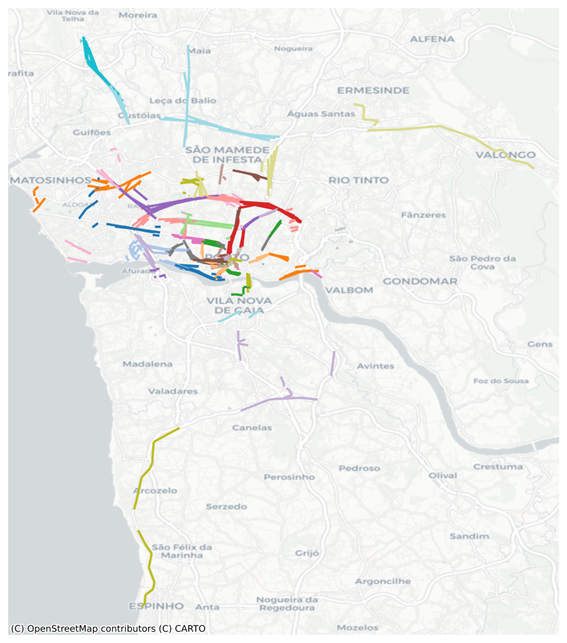
\includegraphics[width=0.5\textwidth]{img/clusters_OPTICS.png}
    \caption{Representación de clusters.}
    \label{fig:clusters_OPTICS}
\end{figure}

\begin{figure}[h!]
    \centering
    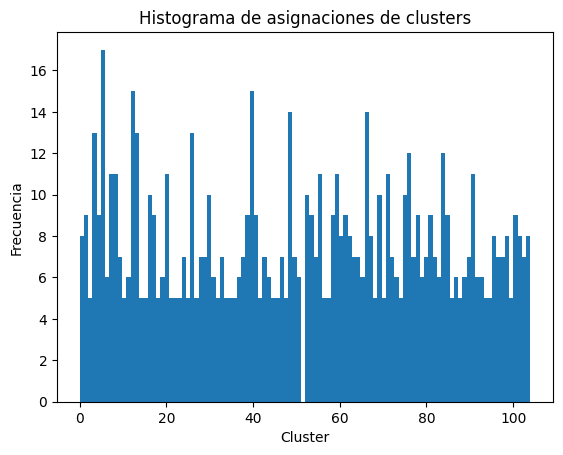
\includegraphics[width=0.5\textwidth]{img/histograma_OPTICS.png}
    \caption{Segmentos por cada cluster.}
    \label{fig:histograma_OPTICS}
\end{figure}

\begin{figure}[h!]
    \centering
    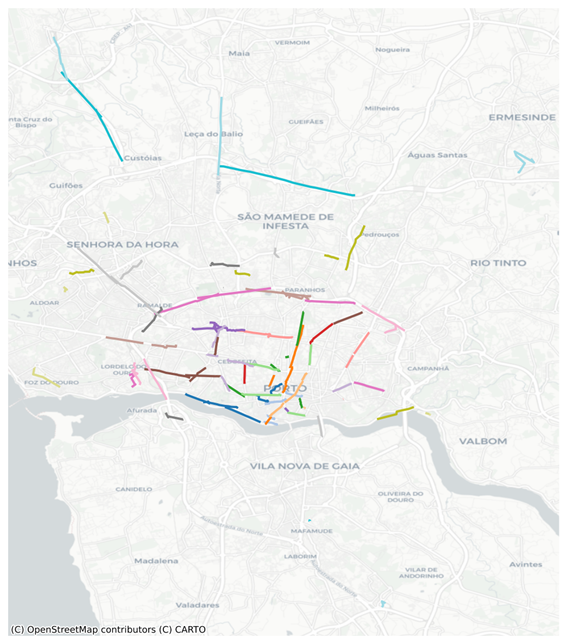
\includegraphics[width=0.5\textwidth]{img/r_tray_OPTICS.png}
    \caption{Representación de trayectorias.}
    \label{fig:trayectorias_OPTICS}
\end{figure}

\FloatBarrier

\item \textbf{DBSCAN}:  
Con un valor de \texttt{eps} de 0.1, los resultados de DBSCAN fueron significativamente diferentes a los de OPTICS. Aunque se generaron más segmentos (2654 en total), el número de clusters disminuyó a 37. Además, el porcentaje de datos clasificados como "basura" aumentó al 90.09\%, lo que equivale a 2391 segmentos descartados.

\begin{figure}[h!]
    \centering
    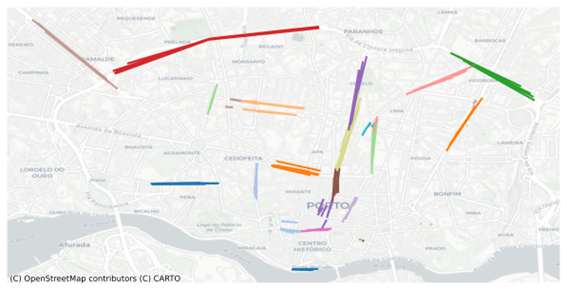
\includegraphics[width=0.5\textwidth]{img/clusters_DBSCAN.png}
    \caption{Representación de clusters.}
    \label{fig:clusters_DBSCAN}
\end{figure}

\begin{figure}[h!]
    \centering
    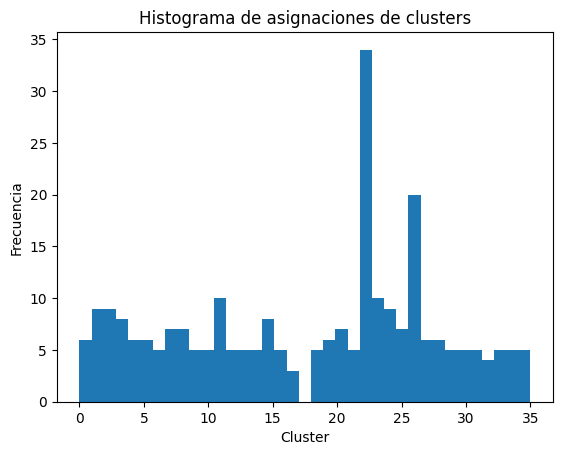
\includegraphics[width=0.5\textwidth]{img/histograma_DBSCAN.png}
    \caption{Segmentos por cada cluster.}
    \label{fig:histograma_DBSCAN}
\end{figure}

\begin{figure}[h!]
    \centering
    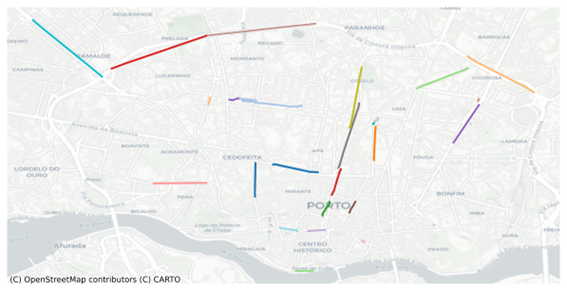
\includegraphics[width=0.5\textwidth]{img/r_tray_DBSCAN.png}
    \caption{Representación de trayectorias.}
    \label{fig:trayectorias_DBSCAN}
\end{figure}

\FloatBarrier

\item \textbf{HDBSCAN}:  
Este algoritmo no requirió ajustes en sus parámetros predeterminados de \texttt{scikit-learn}. Los resultados fueron similares a los de OPTICS en términos de segmentos (2161), aunque el número de clusters fue menor (96) y el porcentaje de segmentos descartados también disminuyó, alcanzando un 53.54\% (1157 segmentos).

\begin{figure}[h!]
    \centering
    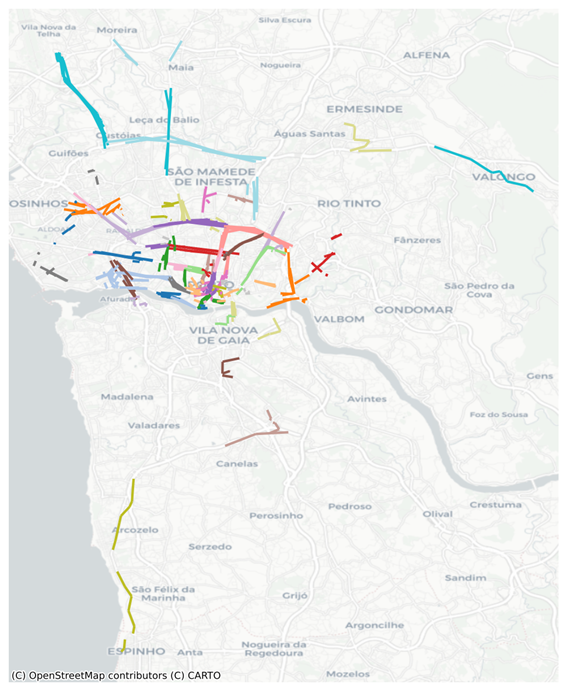
\includegraphics[width=0.5\textwidth]{img/clusters_HDBSCAN.png}
    \caption{Representación de clusters.}
    \label{fig:clusters_HDBSCAN}
\end{figure}

\begin{figure}[h!]
    \centering
    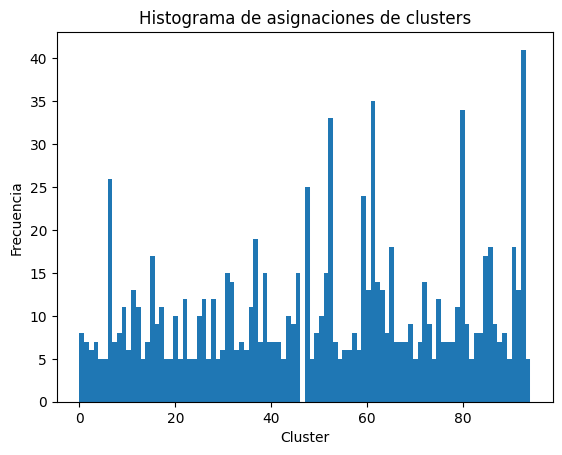
\includegraphics[width=0.5\textwidth]{img/histograma_HDBSCAN.png}
    \caption{Segmentos por cada cluster.}
    \label{fig:histograma_HDBSCAN}
\end{figure}

\begin{figure}[h!]
    \centering
    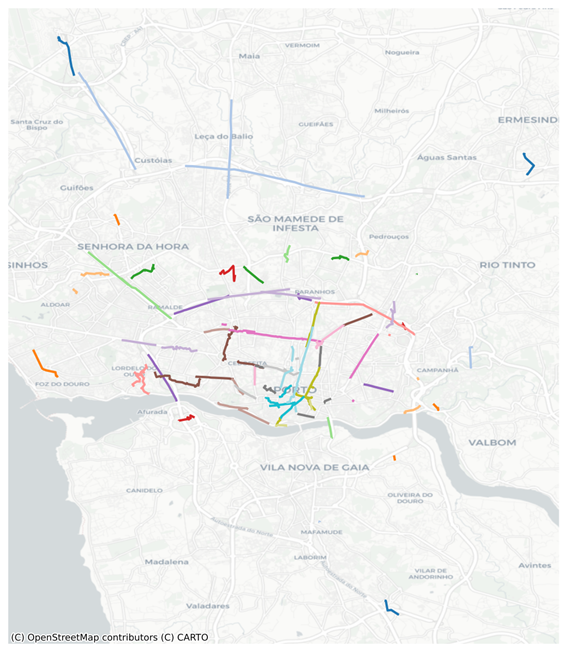
\includegraphics[width=0.5\textwidth]{img/r_tray_HDBSCAN.png}
    \caption{Representación de trayectorias.}
    \label{fig:trayectorias_HDBSCAN}
\end{figure}

\FloatBarrier

\item \textbf{Agglomerative Clustering}:  
Este algoritmo requería definir previamente el número de clusters. En este caso, se utilizaron los 2654 segmentos generados, sin descartar ninguno, ya que no clasifica datos como "basura". Sin embargo, esta característica provoca que los clusters no se centren en las zonas más densas, lo que resulta en representaciones de trayectorias más erráticas.

\begin{figure}[h!]
    \centering
    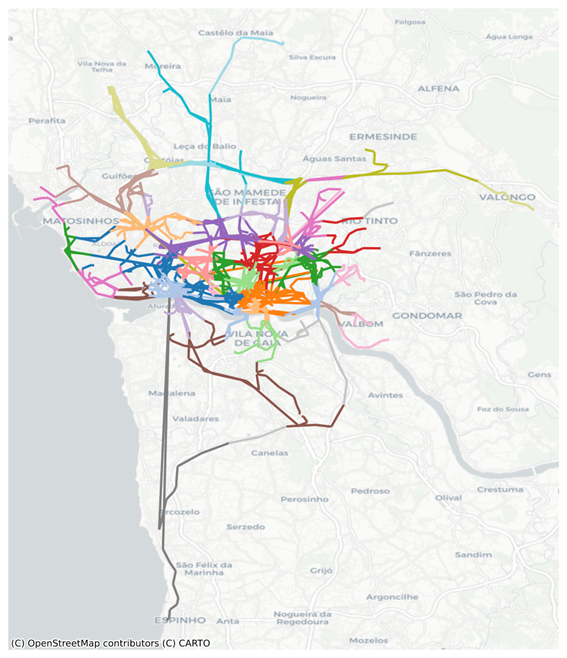
\includegraphics[width=0.5\textwidth]{img/clusters_Aggl.png}
    \caption{Representación de clusters.}
    \label{fig:clusters_Agglomerative}
\end{figure}

\begin{figure}[h!]
    \centering
    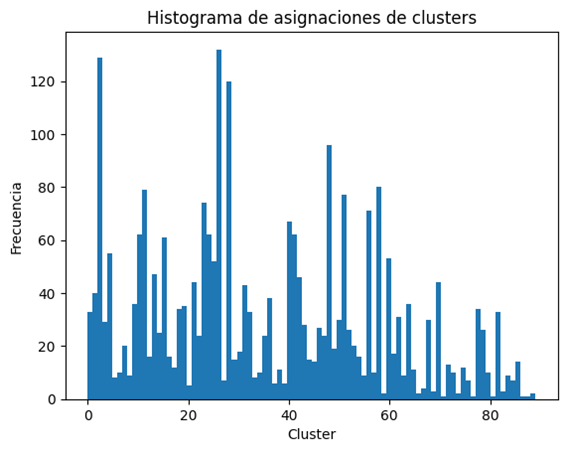
\includegraphics[width=0.5\textwidth]{img/histograma_Aggl.png}
    \caption{Segmentos por cada cluster.}
    \label{fig:histograma_Agglomerative}
\end{figure}

\begin{figure}[h!]
    \centering
    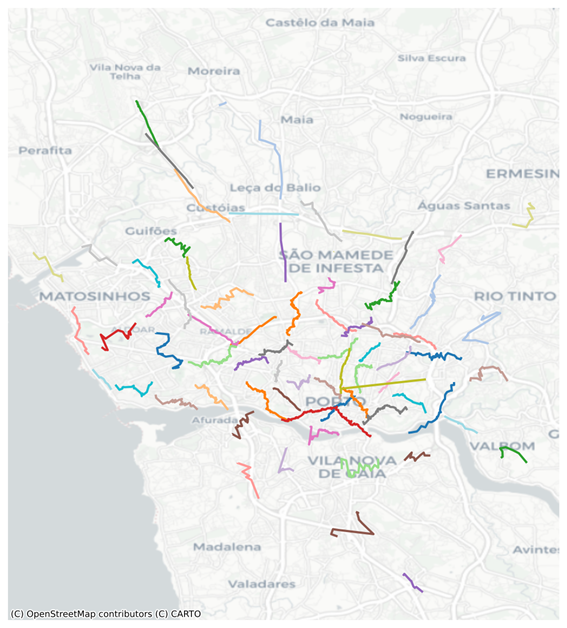
\includegraphics[width=0.5\textwidth]{img/r_tray_Aggl.png}
    \caption{Representación de trayectorias.}
    \label{fig:trayectorias_Agglomerative}
\end{figure}

\FloatBarrier

\item \textbf{Spectral Clustering}:  
Al igual que el algoritmo anterior, no descarta datos. Aunque se generaron los mismos 2654 segmentos y clusters que en Agglomerative Clustering, los resultados finales fueron diferentes, con una distribución menos centralizada.

\begin{figure}[h!]
    \centering
    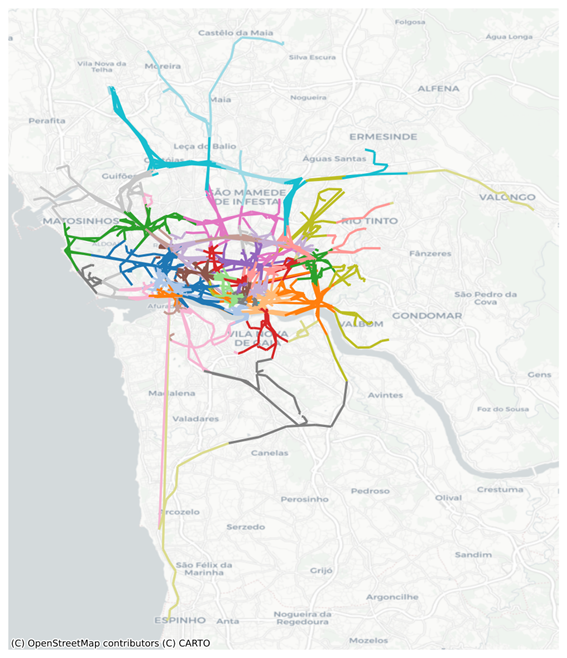
\includegraphics[width=0.5\textwidth]{img/clusters_Spect.png}
    \caption{Representación de clusters.}
    \label{fig:clusters_Spectral}
\end{figure}

\begin{figure}[h!]
    \centering
    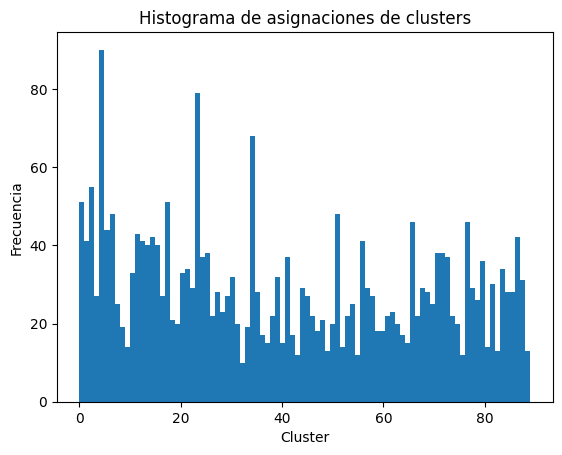
\includegraphics[width=0.5\textwidth]{img/histograma_Spect.png}
    \caption{Segmentos por cada cluster.}
    \label{fig:histograma_Spectral}
\end{figure}

\begin{figure}[h!]
    \centering
    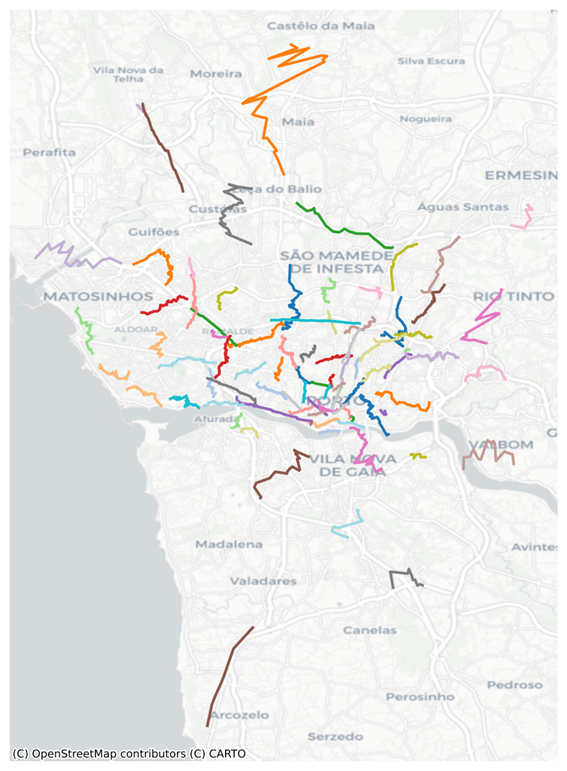
\includegraphics[width=0.5\textwidth]{img/r_tray_Spect.png}
    \caption{Representación de trayectorias.}
    \label{fig:trayectorias_Spectral}
\end{figure}

\FloatBarrier

\end{enumerate}

\subsection{Optimización de la página web} 

Tras múltiples ejecuciones de la página web para comparar los resultados de los diferentes algoritmos de clustering aplicados al TRACLUS, se identificó un problema recurrente: el tiempo de ejecución elevado.

En la aplicación, se podían ejecutar hasta cinco veces consecutivas el algoritmo TRACLUS, cada vez con modificaciones en el algoritmo de clustering. Esta ejecución lineal incrementaba significativamente los tiempos, ya que incluso con pocos datos, el algoritmo mostraba lentitud.

\subsubsection{Estrategia inicial: Uso de hilos}
Para abordar este problema, se reutilizó una estrategia previamente implementada: el uso de hilos. En el controlador \texttt{clustering.py}, que ya gestionaba correctamente el flujo de carga de datos, se dividió el código en funciones separadas, una por cada algoritmo de clustering. Estas funciones eran llamadas según las selecciones del usuario mediante la biblioteca \texttt{threading}.

\subsubsection{Problemas con la generación de mapas y tablas}
Posteriormente, se intentó incorporar la creación de mapas y tablas a estos hilos. Sin embargo, surgieron incompatibilidades con la biblioteca \texttt{matplotlib}, que no es compatible con librerías de hilos como \texttt{concurrent.futures} o \texttt{threading}. Por este motivo, se decidió separar estas tareas. Una vez finalizados todos los hilos, se invocaba una nueva función encargada de generar los mapas necesarios para visualizar los datos.

\subsubsection{Limitaciones de Python}
Aunque esta optimización redujo el tiempo de ejecución, los resultados no alcanzaron las expectativas iniciales. Se identificó que la principal limitación era Python. Su configuración interna impide utilizar múltiples núcleos del procesador de manera eficiente, lo que restringía la velocidad máxima en dispositivos locales. Sin embargo, estas limitaciones no afectaban significativamente la aplicación en entornos remotos, donde el alto rendimiento no era una prioridad debido a los costes asociados.

\subsubsection{Exploración de alternativas de paralelización}
Dado el potencial escalamiento de la aplicación, se exploraron otras estrategias de paralelización:
- \texttt{asyncio}: Diseñada para tareas intensivas en I/O, pero no adecuada para este caso.
- \texttt{Batch Processing}: Orientada a flujos simples, tampoco era aplicable.
- \texttt{Dask} y \texttt{ProcessPoolExecutor}: Ambas opciones cumplían con los requisitos del proyecto.

Se optó por \texttt{ProcessPoolExecutor} debido a su menor complejidad y capacidad para ejecutar funciones en diferentes núcleos del procesador.

\subsubsection{Optimización del flujo de datos}
Además del uso de \texttt{multiprocessing}, se unificó el flujo de representación de los datos en las funciones de multiproceso, lo que resolvió incompatibilidades previas con \texttt{matplotlib}. Esto incrementó considerablemente el rendimiento, ya que anteriormente estas tareas se ejecutaban en serie.

\subsubsection{Resultados obtenidos}
Tras implementar estas mejoras, se lograron resultados significativos:
- \textbf{Operaciones singulares}: La ejecución de un solo TRACLUS con 100 filas de datos pasó de 312 segundos a 288 segundos.
- \textbf{Ejecuciones simultáneas}: La ejecución de cinco TRACLUS con sus respectivos algoritmos de clustering se redujo drásticamente, de 1800 segundos a 450 segundos.

Esta optimización no solo mejoró el rendimiento, sino que también eliminó errores previamente asociados al uso de hilos.


\section{Despliegue de la aplicación}

Para que la aplicación web funcionase correctamente y otros usuarios pudieran utilizarla, era necesario desplegarla desde el entorno local a un entorno de producción. Existen dos formas principales de realizar este proceso: crear un servidor propio o subir la aplicación a un servidor en la nube proporcionado por un tercero. Por razones económicas, se decidió optar por la segunda opción y utilizar un servidor en la nube. Para ello, se exploraron diversos servicios compatibles con aplicaciones basadas en Python.

Entre las opciones evaluadas se encontraron AWS, Azure, Heroku y Conduktor. Aunque muchas de estas plataformas ofrecían soluciones robustas con buen rendimiento, todas presentaban limitaciones económicas, ya que sus funcionalidades avanzadas suelen estar asociadas a costos recurrentes. Esto nos llevó a buscar servicios que ofrecieran una base gratuita que cubriese nuestras necesidades principales.

\subsection{Render: la solución elegida}

Tras evaluar diferentes opciones, se decidió utilizar \textbf{Render}, una plataforma que permite el despliegue de aplicaciones web, APIs y otros servicios. Render ofrece un plan gratuito que resulta ideal para proyectos pequeños o de desarrollo inicial, lo que lo convierte en una opción atractiva para aquellos con presupuestos limitados.

Render proporciona varias ventajas para aplicaciones como la nuestra:
\begin{itemize}
    \item \textbf{Compatibilidad con Python:} Es compatible con aplicaciones basadas en frameworks como Dash, Flask o Django.
    \item \textbf{Despliegue automático:} Permite integrar repositorios de GitHub o GitLab para desplegar automáticamente los cambios realizados en el código.
    \item \textbf{Certificados SSL gratuitos:} Render ofrece certificados de seguridad SSL para garantizar conexiones seguras.
    \item \textbf{Facilidad de configuración:} La plataforma cuenta con una interfaz intuitiva y bien documentada, lo que facilita el proceso de configuración incluso para usuarios con experiencia limitada en despliegues.
    \item \textbf{Soporte para aplicaciones persistentes:} Render soporta aplicaciones que requieren bases de datos o almacenamiento adicional, ideal para aplicaciones web interactivas.
\end{itemize}

\subsection{Proceso de despliegue en Render}

El despliegue de la aplicación en Render se realizó siguiendo los pasos descritos a continuación:

\begin{enumerate}
    \item \textbf{Preparación del repositorio:}
    \begin{itemize}
        \item El proyecto ya estaba alojado en un repositorio de GitHub, se incluyo un archivo \texttt{requirements.txt} que especifica las dependencias necesarias para ejecutar la aplicación.
    \end{itemize}

    \item \textbf{Creación del servicio en Render:}
    \begin{itemize}
        \item Se creó una cuenta gratuita en Render.
        \item Desde el panel de control, se seleccionó la opción \textit{"New Web Service"} y se vinculó el repositorio de GitHub al servicio.
    \end{itemize}

    \item \textbf{Configuración del entorno:}
    \begin{itemize}
        \item Se especificó el comando de inicio de la aplicación, como \texttt{python code/app/main.py}.
        \item Se configuraron las variables de entorno necesarias, como claves API o configuraciones específicas de la aplicación.
    \end{itemize}

    \item \textbf{Despliegue automático:}
    \begin{itemize}
        \item Render detectó automáticamente el contenido del repositorio y comenzó el proceso de construcción e implementación.
        \item Una vez finalizado el proceso, se asignó una URL pública para acceder a la aplicación.
    \end{itemize}

    \item \textbf{Pruebas en producción:}
    \begin{itemize}
        \item Se realizaron pruebas para verificar que todas las funcionalidades de la aplicación estuvieran operativas y que no existieran problemas relacionados con dependencias o configuración.
    \end{itemize}
\end{enumerate}

\subsection{Consideraciones finales}

Aunque Render presenta ciertas limitaciones en su plan gratuito, como tiempos de inicio más lentos para aplicaciones en estado \textit{idle} y límites de recursos, estas no afectaron significativamente a nuestra aplicación durante el desarrollo. La elección de Render permitió concentrar esfuerzos en mejorar la funcionalidad y la experiencia del usuario, sin la necesidad de invertir en infraestructura de servidor.

Con el despliegue en Render, la aplicación quedó lista para ser utilizada por cualquier usuario con acceso a Internet, cumpliendo así el objetivo de trasladar el trabajo desde un entorno local a un entorno accesible y escalable en la nube.

\section{Pruebas funcionales}

Para demostrar la utilidad del algoritmo y la aplicación creados, se propuso realizar múltiples pruebas con diferentes conjuntos de datos, tamaños y configuraciones aplicados a los algoritmos de clustering.

\subsection{Conjuntos de datos}

Durante el desarrollo del proyecto, se utilizó en prácticamente todo el conjunto de datos de Trayectorias Taxis \cite{trayectorias_taxis}. Para esta comprobación final, esto no era suficiente. Usar solo este conjunto de datos limitaría el proyecto a un análisis específico. Por lo tanto, se buscó encontrar múltiples conjuntos de datos cuyo único requisito fuera contener una columna con coordenadas en formato JSON de la siguiente forma: 
[\texttt{[[latitud\_1, longitud\_1], [latitud\_2, longitud\_2], \dots]}]
y que el nombre de dicha columna fuera \texttt{POLYLINE}.

Al no encontrar conjuntos de datos con esta estructura exacta, se decidió adaptar otros conjuntos más comunes que incluyeran coordenadas geográficas en una columna. 

El primer conjunto con esa estructura adaptada fue Geolife \cite{geolife_trajectories}. Este estudio organiza los datos en carpetas, una por cada sujeto al que se le registraron ubicaciones durante un periodo de tiempo. Dentro de cada carpeta se encontraban varios archivos \texttt{.plt} que contenían información sobre la latitud, longitud, hora y fecha de las mediciones. 

Para organizar los datos de forma lógica para el algoritmo TRACLUS, no era viable crear una fila por cada archivo \texttt{.plt}, ya que algunos contenían más de 1000 mediciones. Por lo tanto, se decidió agrupar las mediciones por hora. Todas las mediciones tomadas dentro de la misma hora se combinaron en una única fila de un archivo Excel.

Se creó una función para automatizar este proceso por carpeta, lo que permitió realizar pruebas fácilmente en diferentes sujetos. Para analizar los resultados, se utilizó un archivo Excel generado con todos los datos encontrados en la carpeta del sujeto \texttt{000}.

Otro conjunto de datos probado fue uno de MoveBank \cite{movebank}, una plataforma que contiene miles de trayectorias de animales. Debido a la inmensidad de opciones disponibles, se seleccionó de forma semi-aleatoria el conjunto de datos titulado \textit{"Hammer-headed fruit bats (Hypsignathus monstrosus) in the Republic of Congo"}. Este conjunto incluía datos de múltiples murciélagos de la fruta registrados en diferentes días. 

Tras analizar el número de mediciones por hora, se decidió dividir las trayectorias por murciélago y día, creando un conjunto de datos con filas más reducidas en comparación al anterior. Aun así, estas filas eran considerablemente más grandes que las del conjunto de Trayectorias Taxis, lo cual incrementó significativamente el tiempo de procesamiento por cada fila analizada.

Ademas de estos tres se hicieron pruebas con otros como Citi Bikes \cite{} o Foursquare-NY \cite{} pero aunque organizándonos como los anteriores si que funcionaban se daba la peculiar condicion de que no se generaban los mapas de fondo lo que perdía parte de la razon del estudio, casualmente los dos se hubicaban en los estado unidos, nueva jork, lo que seguramente es la razon auque hasta el momento se habian usado hubicaciones muy diversas, portugal, china y el congo. 

\begin{figure}[h!]
    \centering
    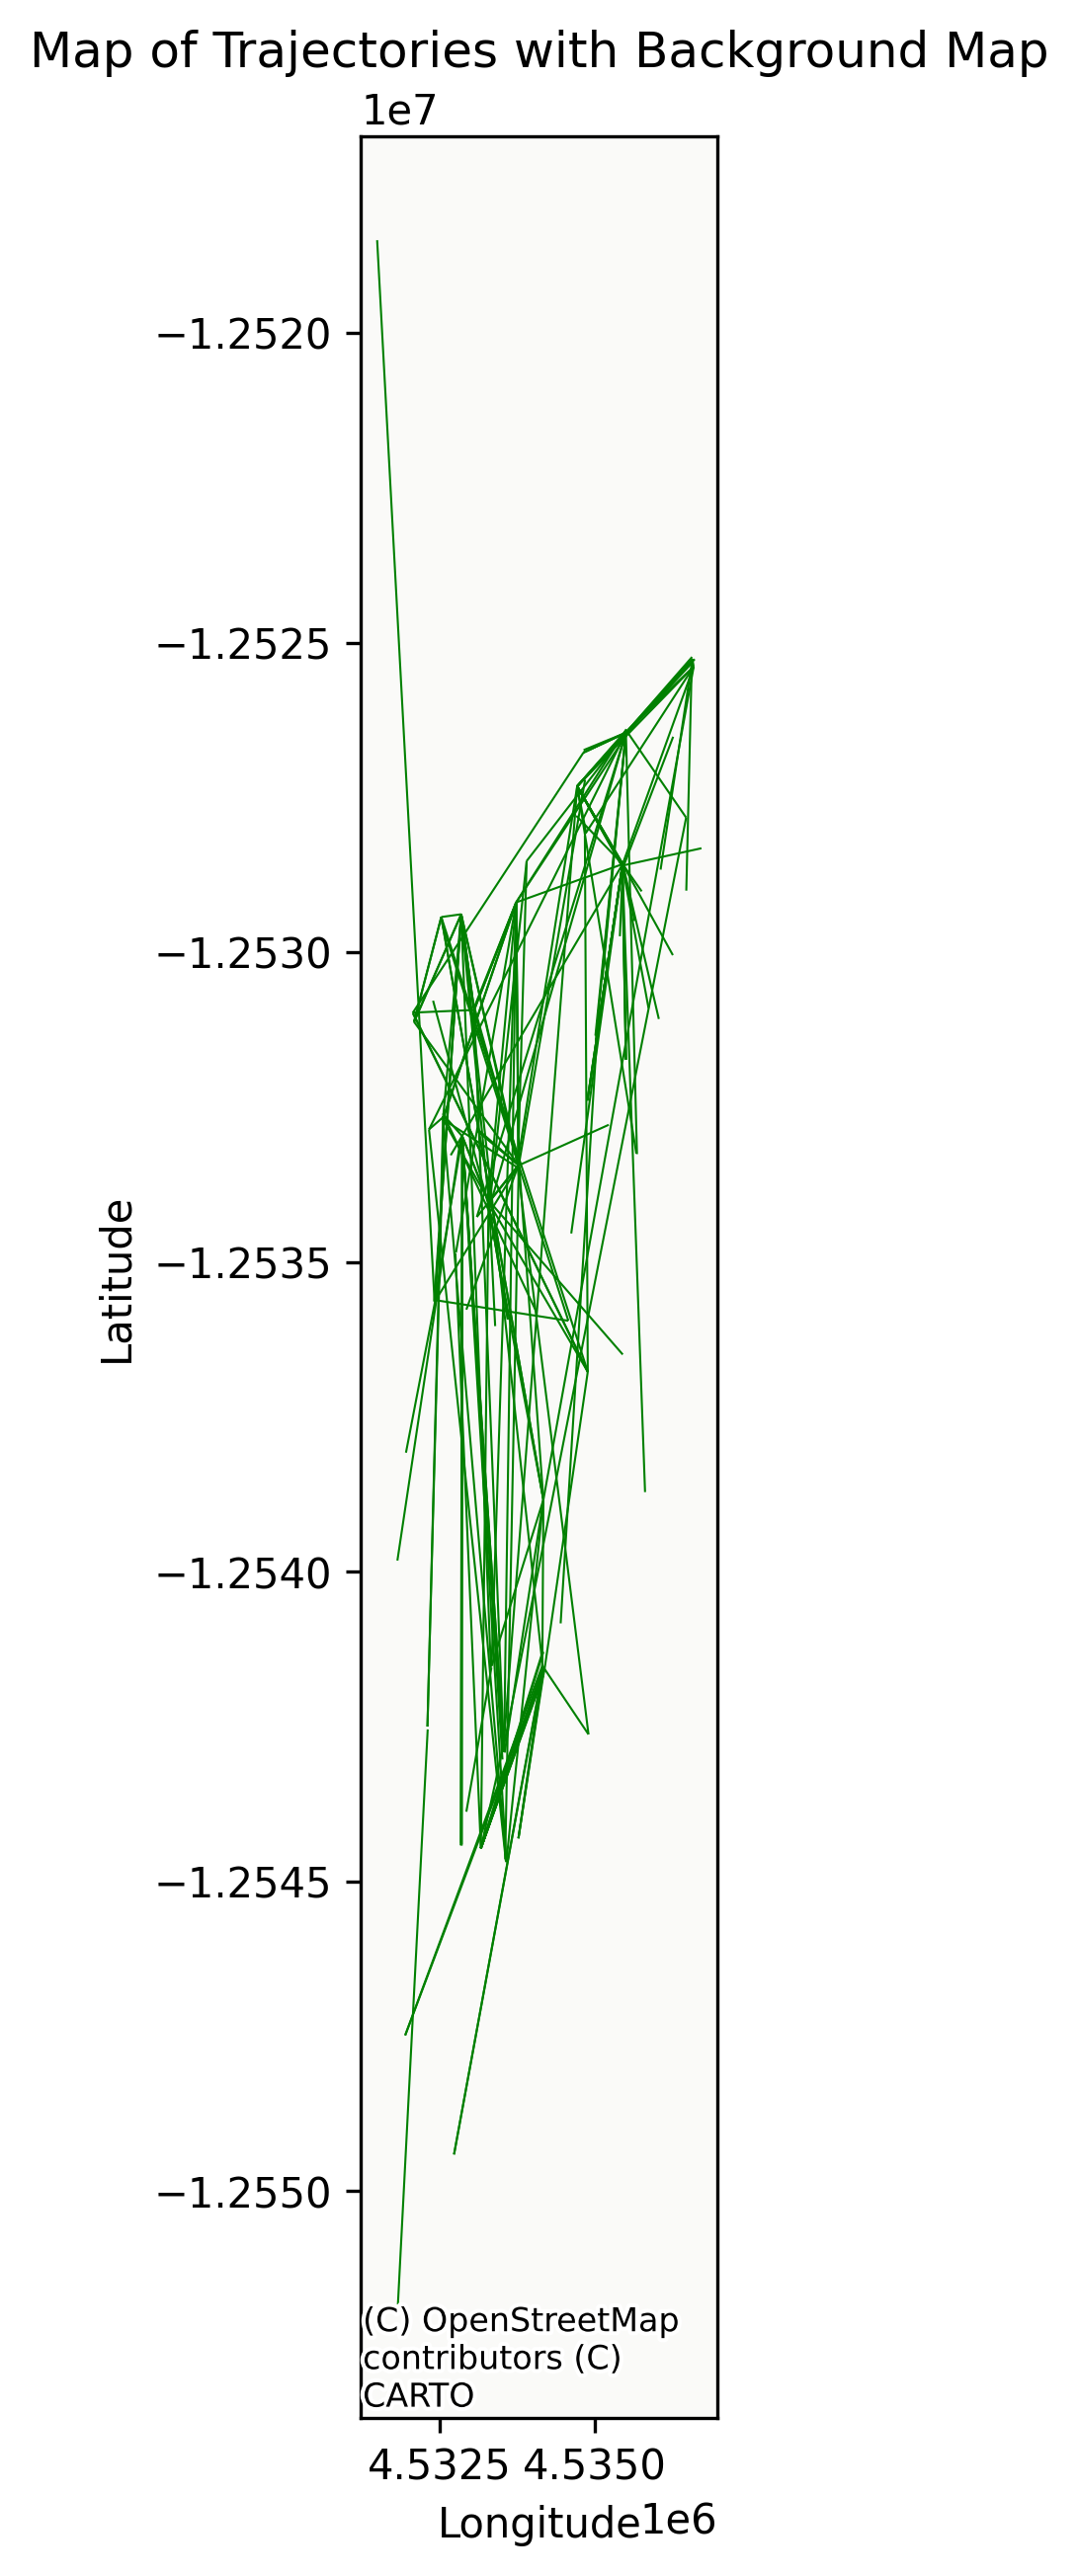
\includegraphics[width=0.5\textwidth]{img/CitiBike_trayectories.png}
    \caption{Mapa de trayectorias sin tratar del cojunto Citi Bikes.}
    \label{fig:clusters_Spectral}
\end{figure}

\subsection{Explicación de las pruebas}

Para realizar un análisis coherente del TRACLUS con los diferentes algoritmos de clustering, es esencial definir claramente los objetivos, identificar los parámetros ajustables y establecer los límites de las pruebas. 

El propósito de estas pruebas era comprobar el funcionamiento del programa desarrollado durante el proyecto, evaluar los tiempos de ejecución bajo diversas condiciones y analizar cómo los diferentes parámetros de los algoritmos de clustering impactan los resultados obtenidos.

En cada algoritmo de clustering, existen parámetros configurables que influyen significativamente en los resultados. Los parámetros seleccionados para incluir en la aplicación son aquellos que se consideraron más relevantes para el análisis. A continuación, se explican en detalle los algoritmos y sus parámetros:

\begin{enumerate}
    \item \textbf{OPTICS (Ordering Points To Identify the Clustering Structure):}
    Este algoritmo identifica clusters de diferentes densidades en los datos. Los principales parámetros configurables son:
    \begin{enumerate}
        \item \textbf{Metric:} Define la métrica utilizada para calcular las distancias entre puntos. Las opciones disponibles son:
        \begin{enumerate}
            \item \textbf{euclidean:} Utiliza la distancia euclidiana tradicional.
            \item \textbf{l1:} Calcula la distancia Manhattan.
            \item \textbf{l2:} Similar a euclidean, pero con ajustes para ciertas aplicaciones.
            \item \textbf{manhattan:} Igual que \textit{l1}, mide la distancia entre dos puntos como la suma de sus diferencias absolutas.
            \item \textbf{cosine:} Calcula la similitud basada en el coseno del ángulo entre vectores.
            \item \textbf{cityblock:} Otra forma de describir la distancia Manhattan.
        \end{enumerate}
        \item \textbf{Algorithm:} Selecciona el método para encontrar vecinos más cercanos:
        \begin{enumerate}
            \item \textbf{auto:} Elige automáticamente el método más eficiente según los datos.
            \item \textbf{ball\_tree:} Usa una estructura de árbol espacial para organizar los puntos.
            \item \textbf{kd\_tree:} Similar a \textit{ball\_tree}, pero optimizado para ciertas métricas.
            \item \textbf{brute:} Calcula las distancias directamente, sin estructuras optimizadas.
        \end{enumerate}
        \item \textbf{Max\_eps:} Establece el radio máximo para considerar puntos vecinos.
        \item \textbf{Min\_samples:} Define el número mínimo de puntos necesarios para formar un cluster.
    \end{enumerate}
    
    \item \textbf{DBSCAN (Density-Based Spatial Clustering of Applications with Noise):}
    Este algoritmo agrupa puntos densos mientras ignora ruido. Comparte parámetros con OPTICS:
    \begin{enumerate}
        \item \textbf{Metric:} Igual que en OPTICS.
        \item \textbf{Algorithm:} Igual que en OPTICS.
        \item \textbf{Eps:} Especifica el radio para considerar vecinos.
        \item \textbf{Min\_samples:} Igual que en OPTICS.
    \end{enumerate}
    
    \item \textbf{HDBSCAN (Hierarchical Density-Based Spatial Clustering of Applications with Noise):}
    Este algoritmo extiende DBSCAN para trabajar mejor con datos de densidad variable:
    \begin{enumerate}
        \item \textbf{Metric:} Igual que en OPTICS.
        \item \textbf{Algorithm:} Igual que en OPTICS.
        \item \textbf{Min\_samples:} Igual que en OPTICS.
    \end{enumerate}
    
    \item \textbf{Agglomerative Clustering:}
    Este algoritmo agrupa puntos en una jerarquía utilizando diferentes criterios de vinculación:
    \begin{enumerate}
        \item \textbf{Metric:} Igual que en OPTICS.
        \item \textbf{Linkage:} Determina cómo calcular la distancia entre clusters:
        \begin{enumerate}
            \item \textbf{ward:} Minimiza la varianza dentro de los clusters.
            \item \textbf{complete:} Maximiza la distancia entre puntos más lejanos de clusters diferentes.
            \item \textbf{average:} Calcula la distancia media entre todos los puntos de dos clusters.
            \item \textbf{single:} Minimiza la distancia entre los puntos más cercanos de dos clusters.
        \end{enumerate}
        \item \textbf{n\_clusters:} Especifica el número de clusters deseados en los resultados.
    \end{enumerate}
    
    \item \textbf{Spectral Clustering:}
    Este algoritmo utiliza el espectro del grafo de afinidad para realizar clustering:
    \begin{enumerate}
        \item \textbf{Affinity:} Define cómo construir el grafo de afinidad:
        \begin{enumerate}
            \item \textbf{nearest\_neighbors:} Usa vecinos más cercanos para definir las relaciones.
            \item \textbf{rbf:} Utiliza una función base radial para calcular similitudes.
            \item \textbf{precomputed:} Trabaja con una matriz de afinidad ya calculada.
            \item \textbf{precomputed\_nearest\_neighbors:} Usa vecinos más cercanos predefinidos.
        \end{enumerate}
        \item \textbf{Assign\_labels:} Define el método para asignar etiquetas a clusters:
        \begin{enumerate}
            \item \textbf{kmeans:} Usa el algoritmo K-Means para asignar etiquetas.
            \item \textbf{discretize:} Utiliza discretización para asignar etiquetas.
            \item \textbf{cluster\_qr:} Asigna etiquetas usando descomposición QR.
        \end{enumerate}
        \item \textbf{n\_clusters:} Especifica el número de clusters deseados en los resultados.
    \end{enumerate}
\end{enumerate}

Estas pruebas no solo validaron el funcionamiento de la aplicación, sino que también proporcionaron una comprensión más profunda de cómo los diferentes parámetros afectan el comportamiento de los algoritmos en diversos contextos.

\subsubsection*{Criterios para las pruebas:}

\begin{enumerate}
    \item \textbf{Límite de tiempo:} Cada prueba debe durar un máximo de dos horas, considerando tanto el tiempo de ejecución como el de representación de los datos. Este límite puede variar según el tamaño del conjunto de datos y el número de coordenadas procesadas.
    \item \textbf{Selección de parámetros:} No se probarán todas las combinaciones posibles. Se seleccionarán aquellas configuraciones que se consideren más relevantes y que puedan producir cambios significativos en los resultados.
    \item \textbf{Pruebas iniciales intensivas:} Se realizarán pruebas más pesadas al inicio, aunque en menor cantidad, para estimar mejor los tiempos de ejecución y obtener resultados más representativos.
\end{enumerate}

\subsection{Resultados}

Las pruebas iniciaron con un análisis de rendimiento. Primero, se evaluó cómo funcionaría la aplicación al ejecutarse en remoto utilizando Render. Los resultados fueron poco satisfactorios debido a varias limitaciones inherentes a la versión gratuita de Render, tales como un rendimiento bajo y restricciones significativas de memoria. Dado que el programa requiere recursos considerables para procesar correctamente grandes cantidades de datos o ejecutar múltiples algoritmos de clustering de forma simultánea, se produjeron errores al superar la memoria disponible o por tiempos de ejecución excesivos. 

Debido a estas limitaciones económicas, se optó por realizar todas las pruebas de manera local.

\subsubsection{Configuraci\'on inicial}

Se comenzaron las pruebas utilizando diferentes conjuntos de datos y ajustando los parámetros a valores iniciales básicos. Los datos de prueba consistieron en 10 filas de cada conjunto, y se utilizaron los cinco algoritmos de clustering con los siguientes parámetros iniciales:

\begin{itemize}
    \item \textbf{Metric:} \texttt{euclidean}
    \item \textbf{Algorithm:} \texttt{auto}
    \item \textbf{Min\_samples:} 5
    \item \textbf{Max\_eps:} 1
    \item \textbf{Eps:} 0.1
    \item \textbf{Linkage:} \texttt{ward}
    \item \textbf{Affinity:} \texttt{nearest\_neighbors}
    \item \textbf{Assign\_labels:} \texttt{kmeans}
    \item \textbf{n\_clusters:} 7
\end{itemize}

\subsubsection{Análisis de los resultados}

\paragraph{Rendimiento por conjunto de datos}

\begin{itemize}
    \item \textbf{Trayectorias Taxis} \cite{trayectorias_taxis}  \\
    Tiempo de ejecución aproximado: \textbf{45 segundos}.

    \item \textbf{Geolife} \cite{geolife_trajectories} (ordenado por horas)  \\
    Tiempo de ejecución aproximado: \textbf{2 minutos y 50 segundos}.

    \item \textbf{MoveBank} \cite{movebank} (ordenado por día y id)\\
    Tiempo de ejecución aproximado: \textbf{1 minutos y 50 segundos}.
\end{itemize}

\paragraph{Hallazgos preliminares}

\begin{enumerate}
    \item \textbf{OPTICS y HDBSCAN producen resultados similares}  \\
    En los tres conjuntos de datos, los resultados de OPTICS y HDBSCAN fueron idénticos cuando el parámetro \texttt{Max\_eps} se fijó en 1. Esto sugiere que, bajo los parámetros configurados en esta aplicación, ambos algoritmos interactúan de manera muy similar. Esto es consistente con la naturaleza de ambos, ya que son derivados de DBSCAN.

    \item \textbf{Efecto del tamaño de los datos}  \\
    El análisis reveló cómo el tamaño de los datos iniciales afecta los resultados. A continuación, se presentan los resultados específicos para cada conjunto de datos:
\end{enumerate}

\subparagraph{Geolife (10 filas)}

Los resultados iniciales de Geolife mostraron trayectorias extensas y separadas, lo que influyó en los resultados de cada algoritmo:

\begin{figure}[h!]
    \centering
    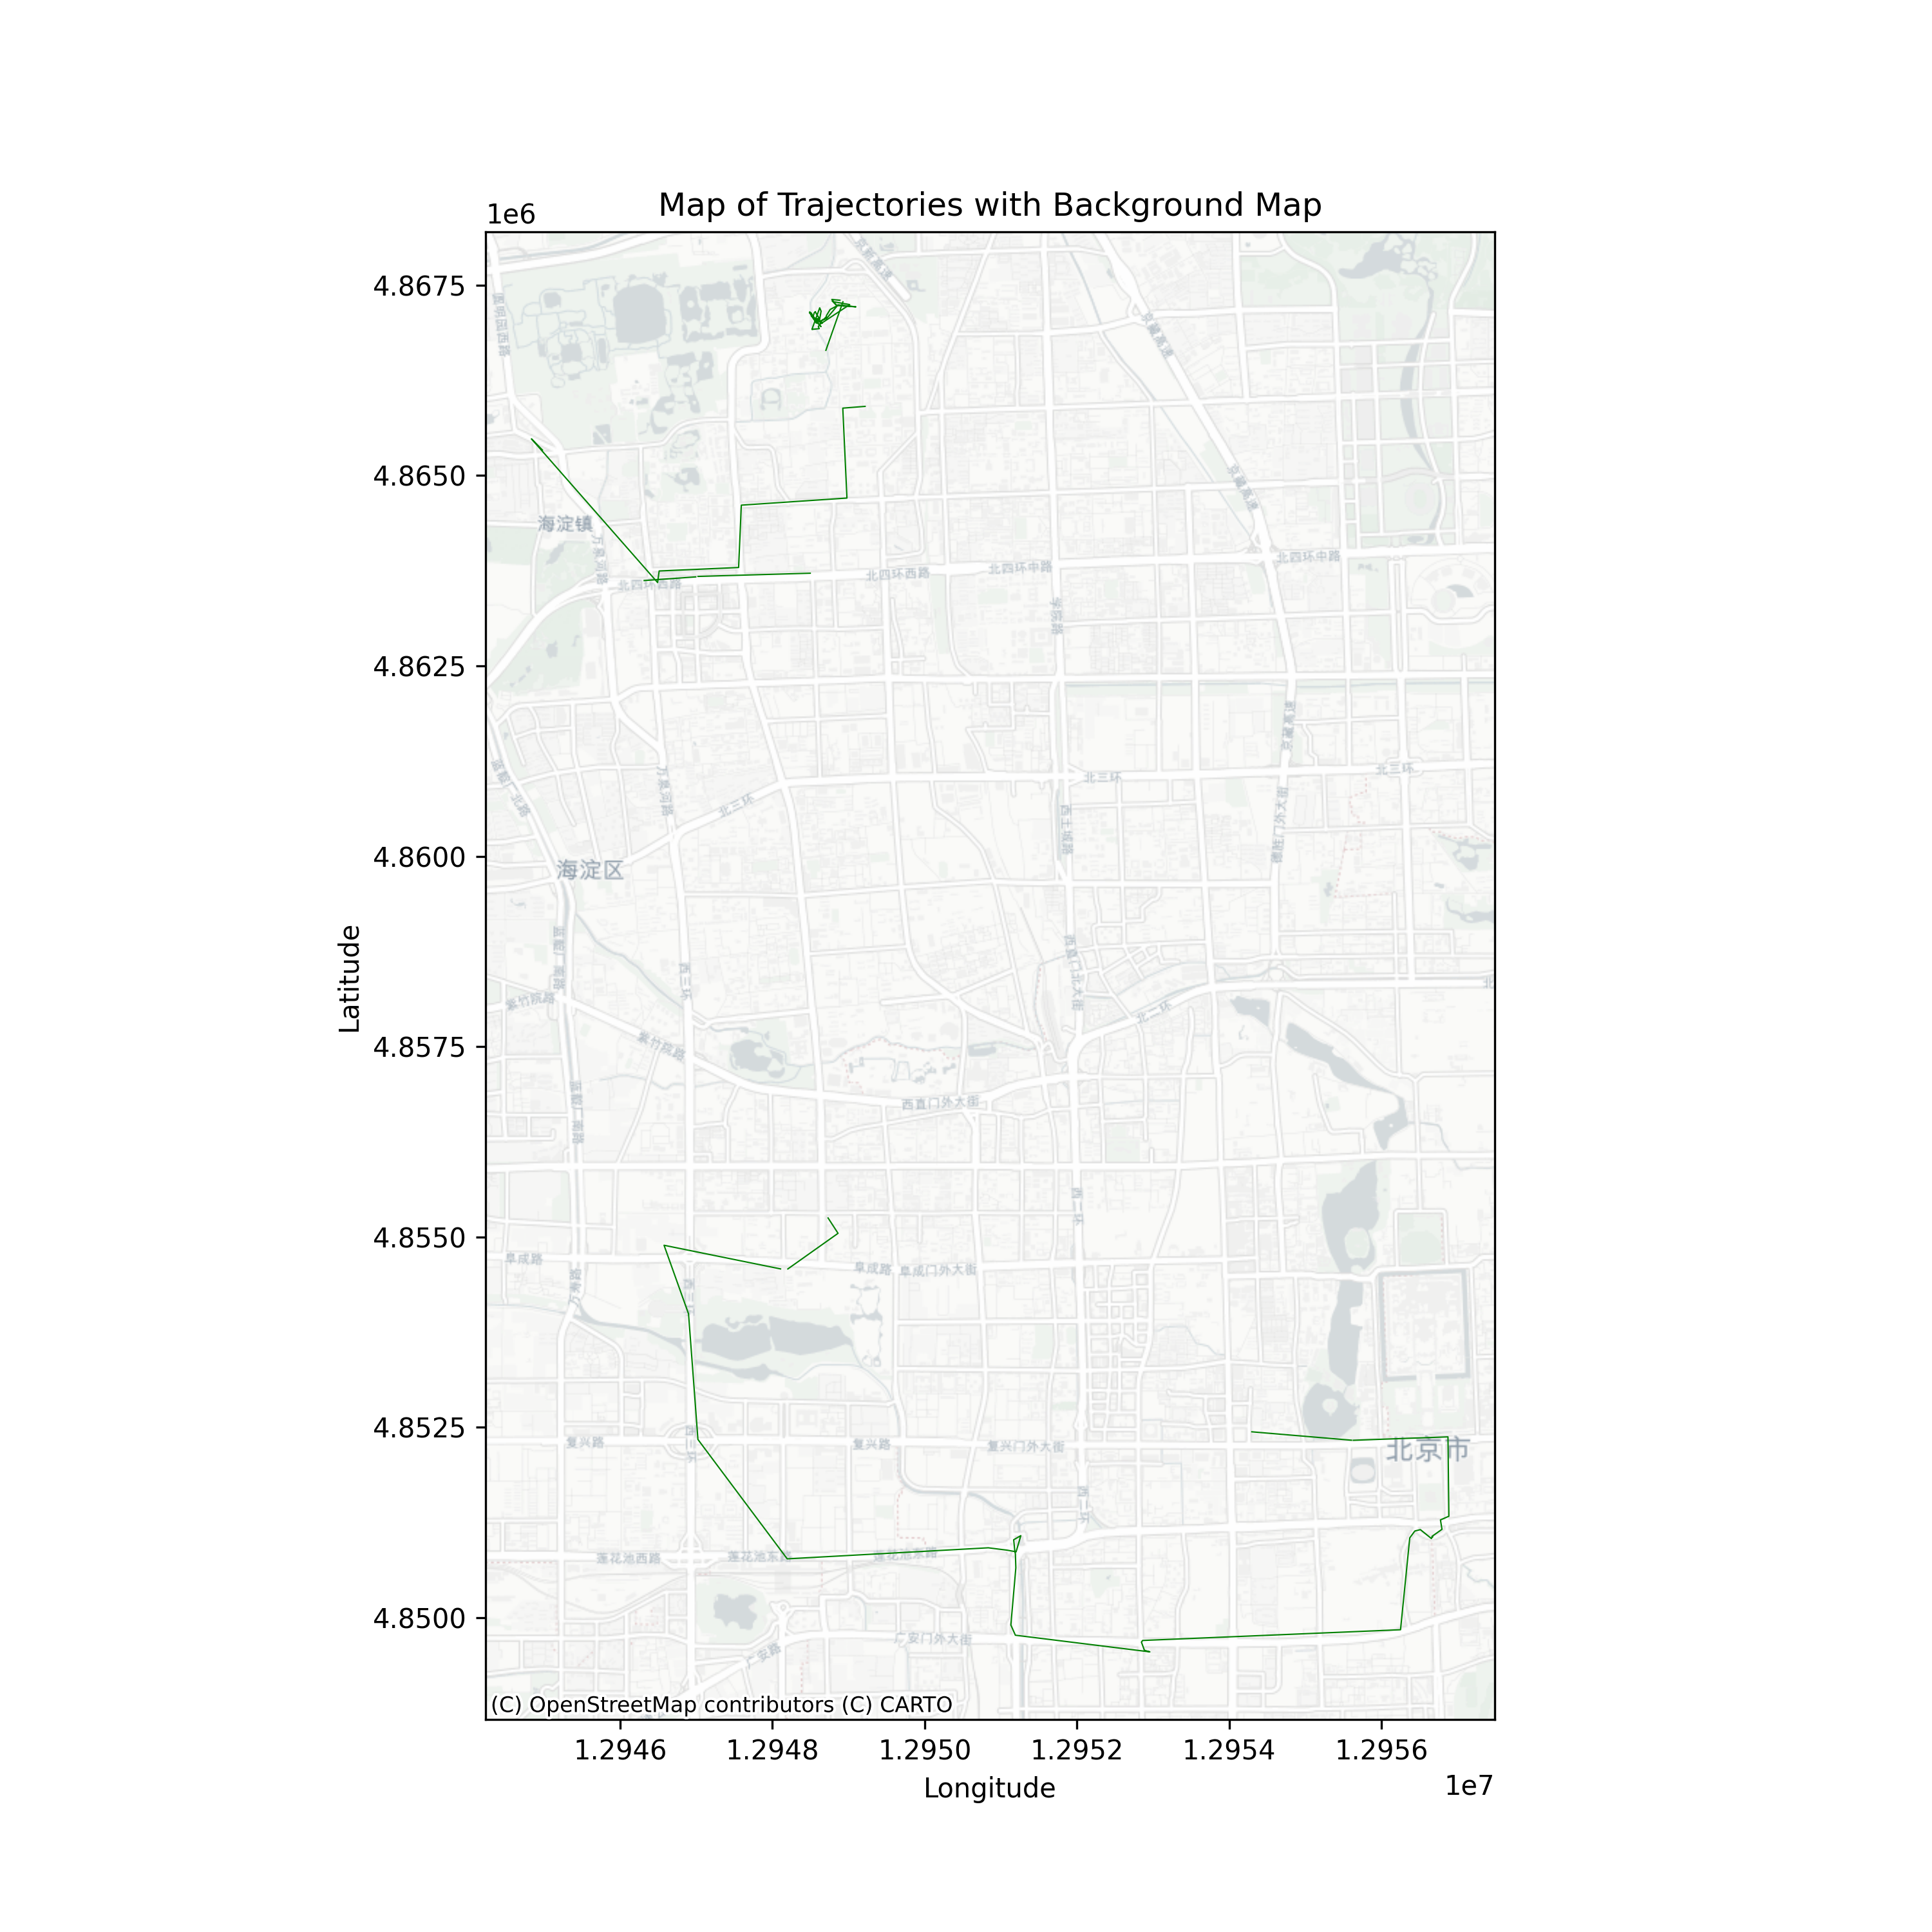
\includegraphics[width=0.5\textwidth]{img/Geolife/map_prueba_10datos.png}
    \caption{Mapa de trayectorias Geolife, 10 filas.}
    \label{fig:geolife_10}
\end{figure}

\begin{itemize}
    \item \textbf{OPTICS y DBSCAN:} Dado que los datos estaban dispersos, estos algoritmos identificaron puntos medios de distancia con poca coherencia.
    
	\begin{figure}[h!]
   		\centering
    		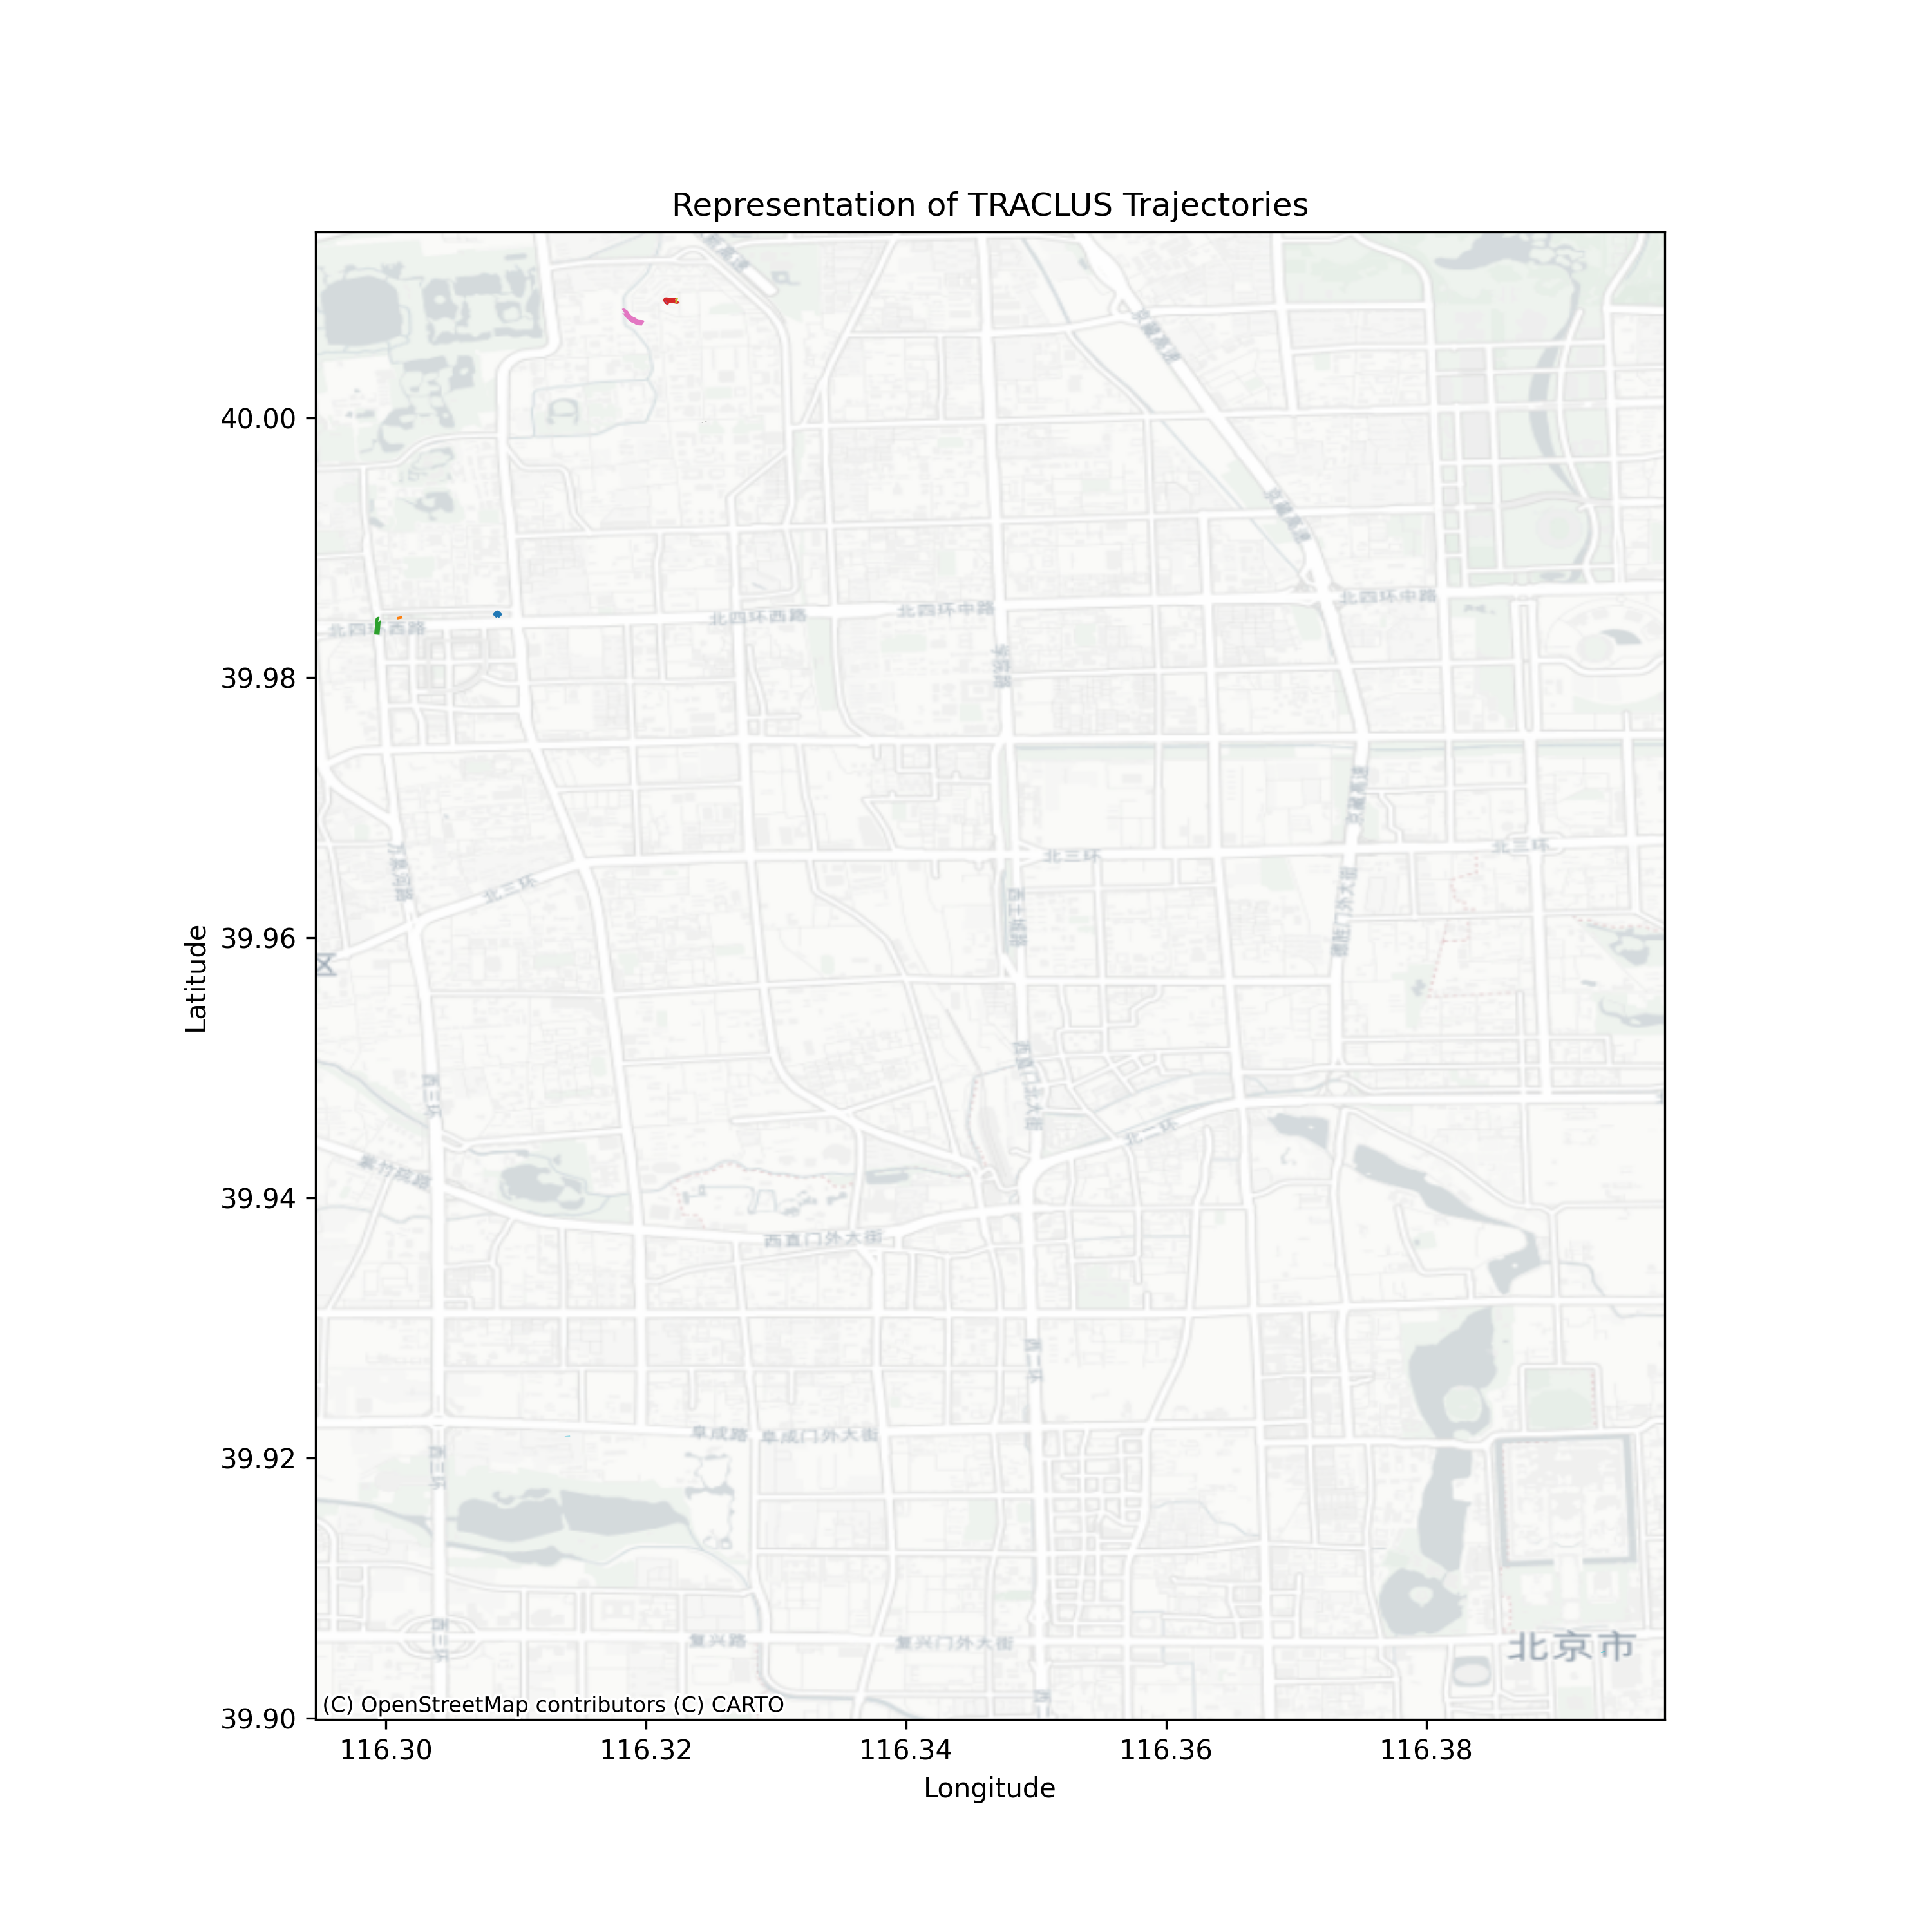
\includegraphics[width=0.5\textwidth]{img/Geolife/map_optics_10datos.png}
    		\caption{Mapa trayectorias resultantes OPTICS y DBSCAN, 10 filas.}
    		\label{fig:geolife_10}
	\end{figure}
    
    \item \textbf{HDBSCAN:} Generó dos trayectorias principales, correspondientes a las zonas donde los movimientos del sujeto se concentraban.

	\begin{figure}[h!]
   		\centering
    		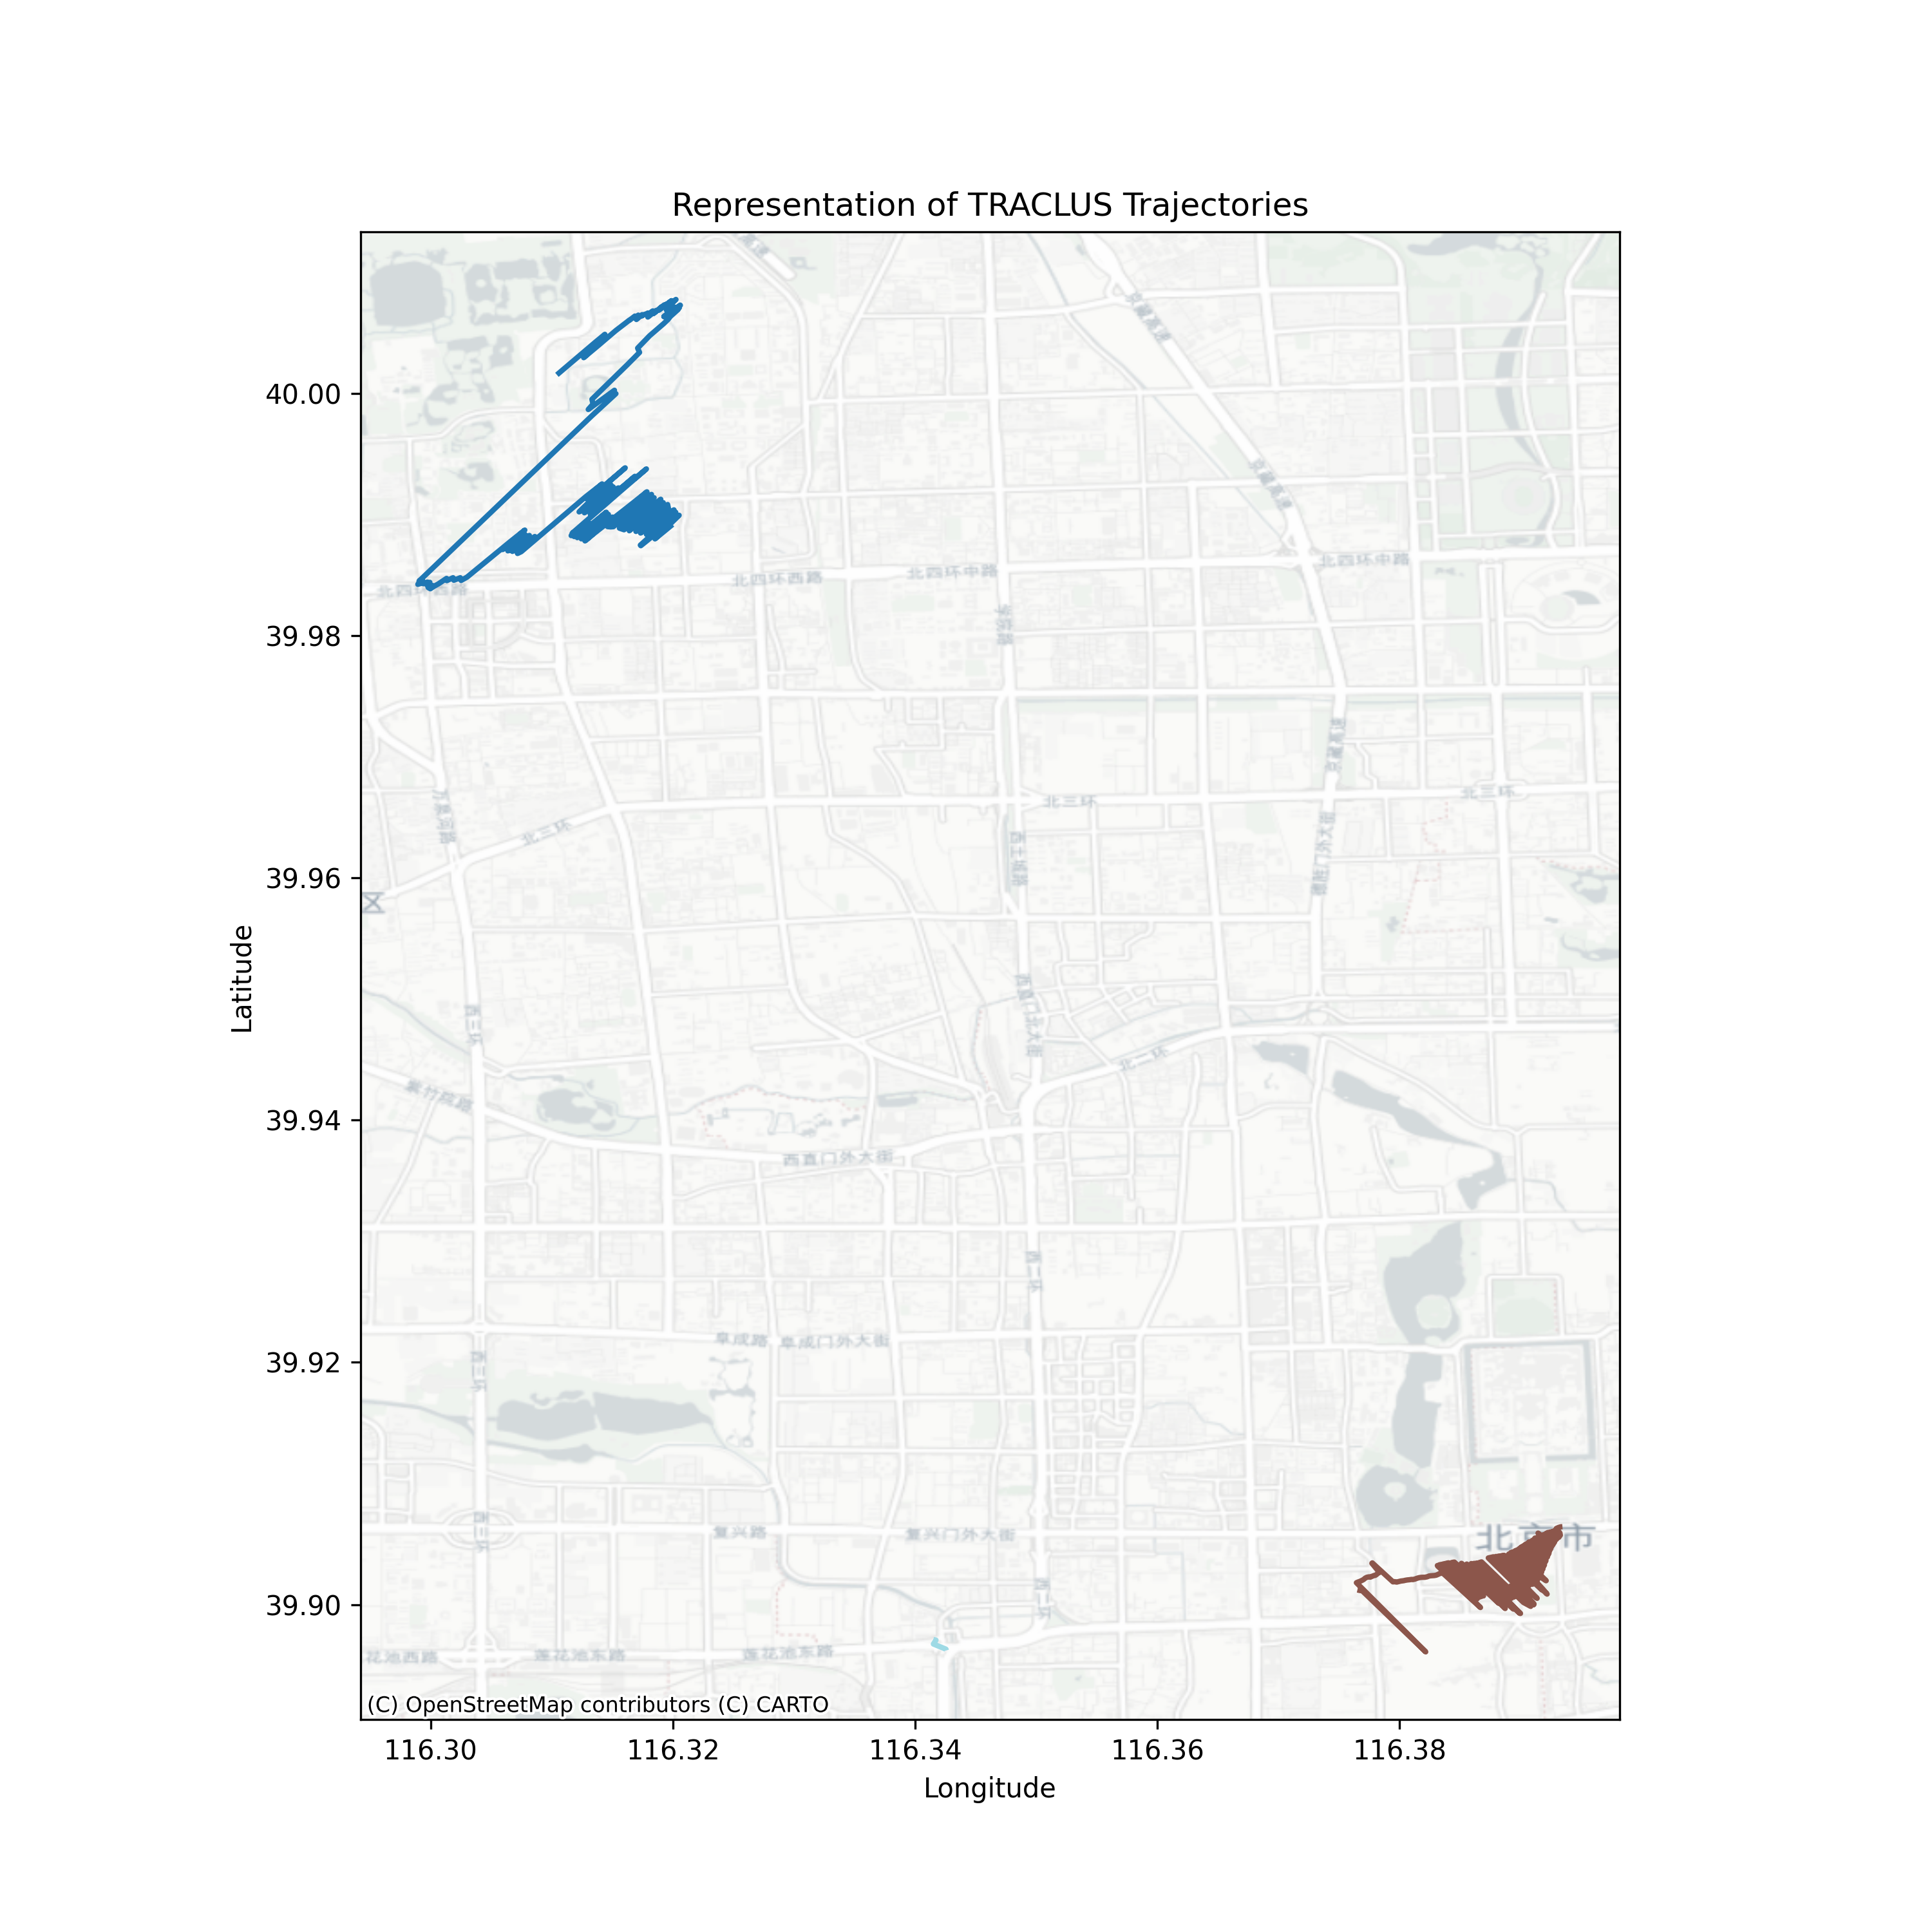
\includegraphics[width=0.5\textwidth]{img/Geolife/map_hdbscan_10datos.png}
    		\caption{Mapa trayectorias resultantes HDBSCAN, 10 filas.}
    		\label{fig:geolife_10}
	\end{figure}    
    
    \item \textbf{Agglomerative Clustering y Spectral Clustering:} Fragmentaron los datos en zonas de interés similar a HDBSCAN, debido a la configuración de \texttt{n\_clusters} en 7.

	\begin{figure}[h!]
   		\centering
    		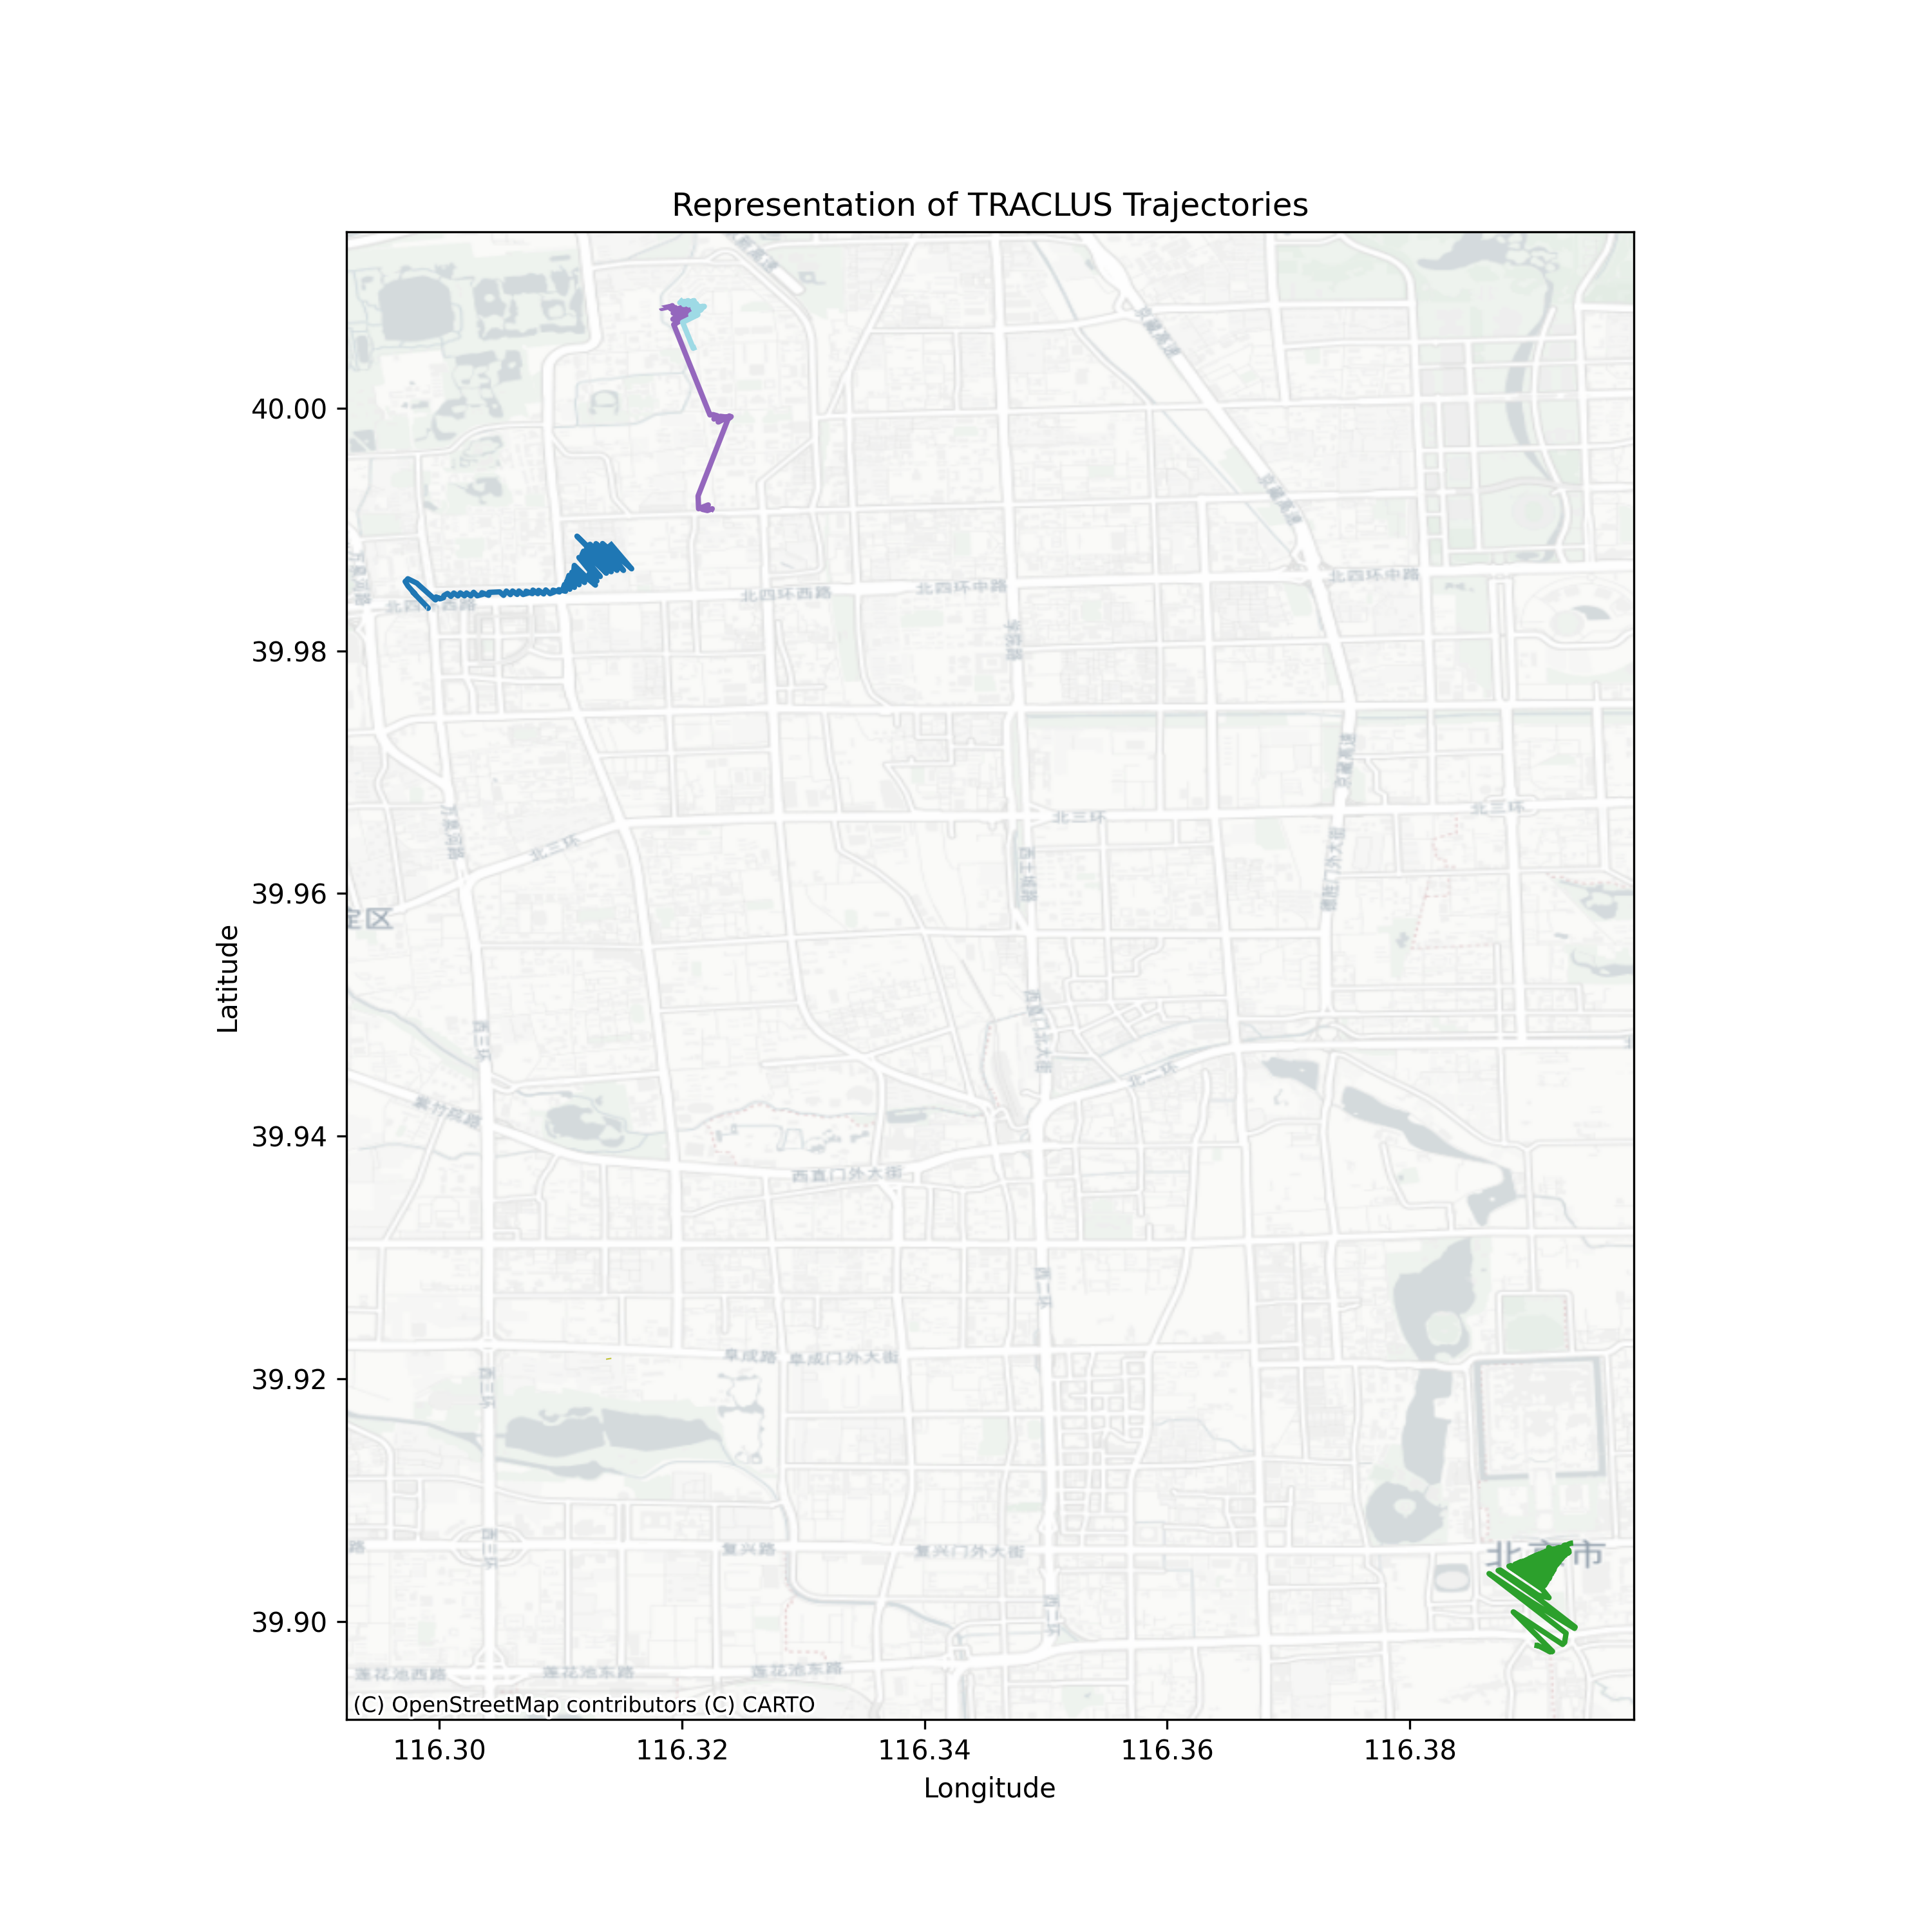
\includegraphics[width=0.5\textwidth]{img/Geolife/map_aggl_10datos.png}
    		\caption{Mapa trayectorias resultantes Agglomerative, 10 filas.}
    		\label{fig:geolife_10}
	\end{figure}
	
	\begin{figure}[h!]
   		\centering
    		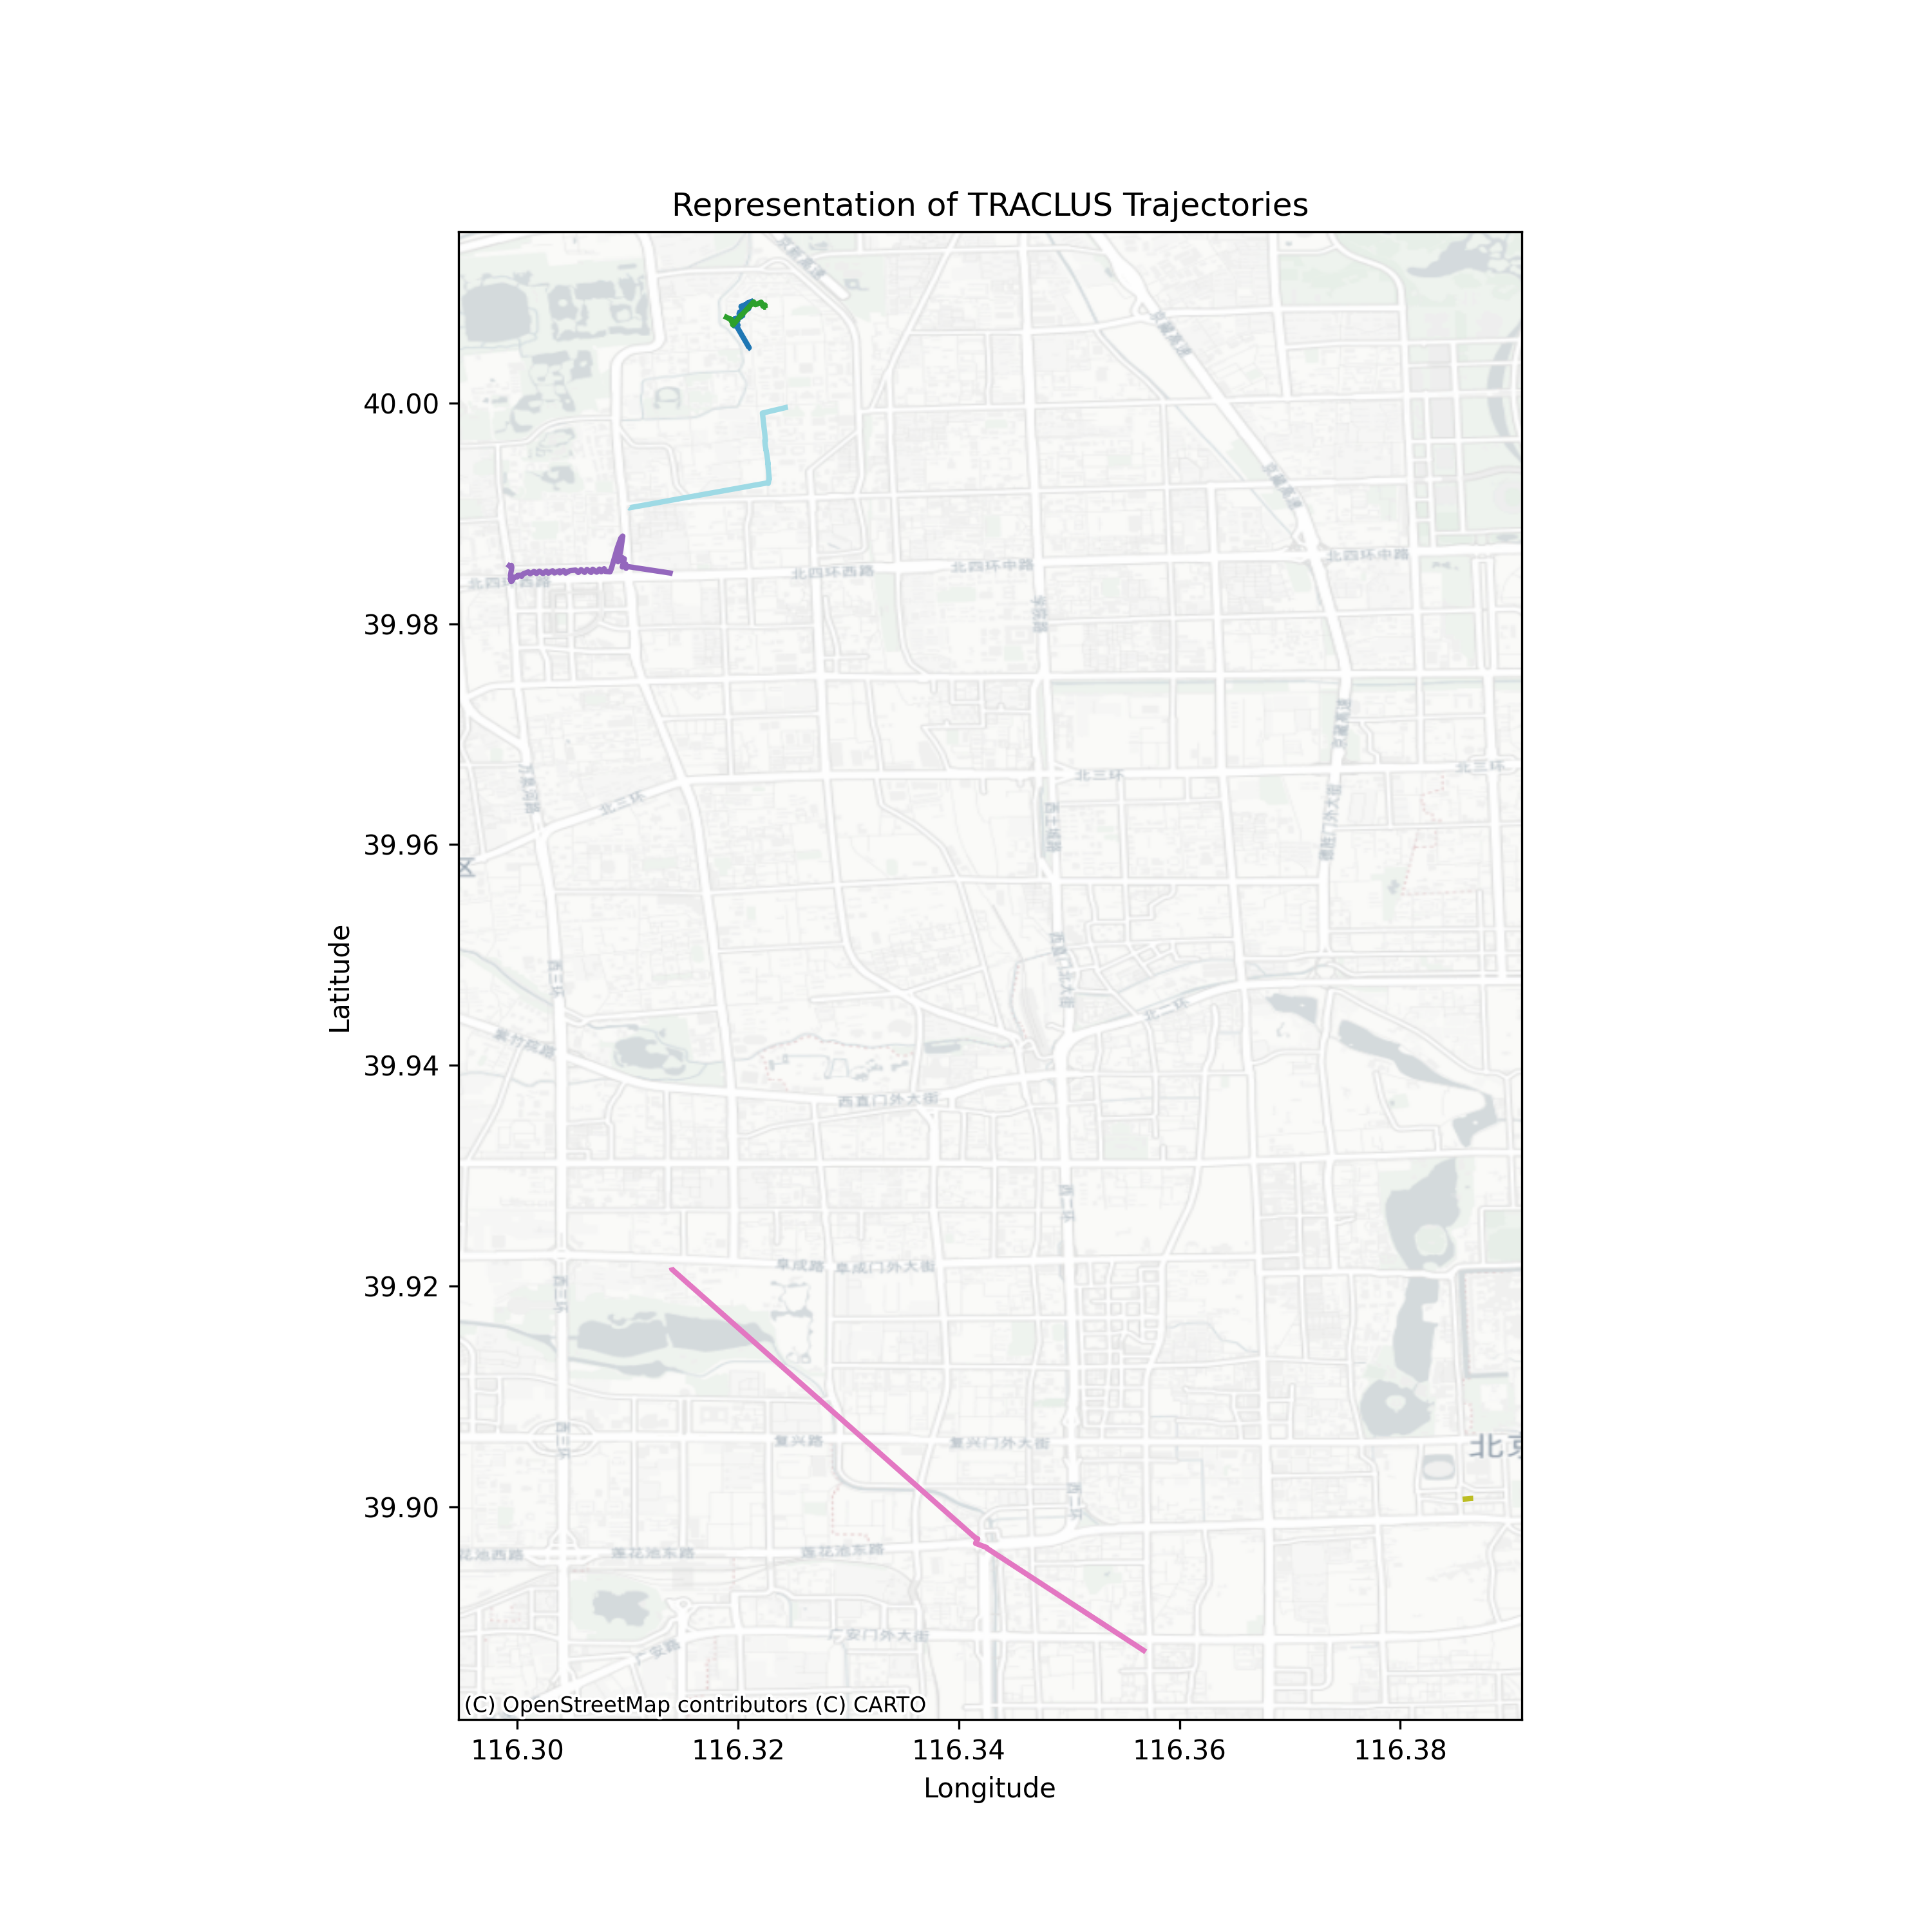
\includegraphics[width=0.5\textwidth]{img/Geolife/map_spect_10datos.png}
    		\caption{Mapa trayectorias resultantes Spectral, 10 filas.}
    		\label{fig:geolife_10}
	\end{figure}    
    
\end{itemize}


\subparagraph{MoveBank (10 filas)}

Este conjunto presentó movimientos concentrados en un área específica, con un desplazamiento esporádico a una gran distancia. Esto produjo que los algoritmos no fueran capaces de mostrar ningún resultado visible al igual que OPTICS Y DBSCAN en el conjunto anterior.

\begin{figure}[h!]
    \centering
    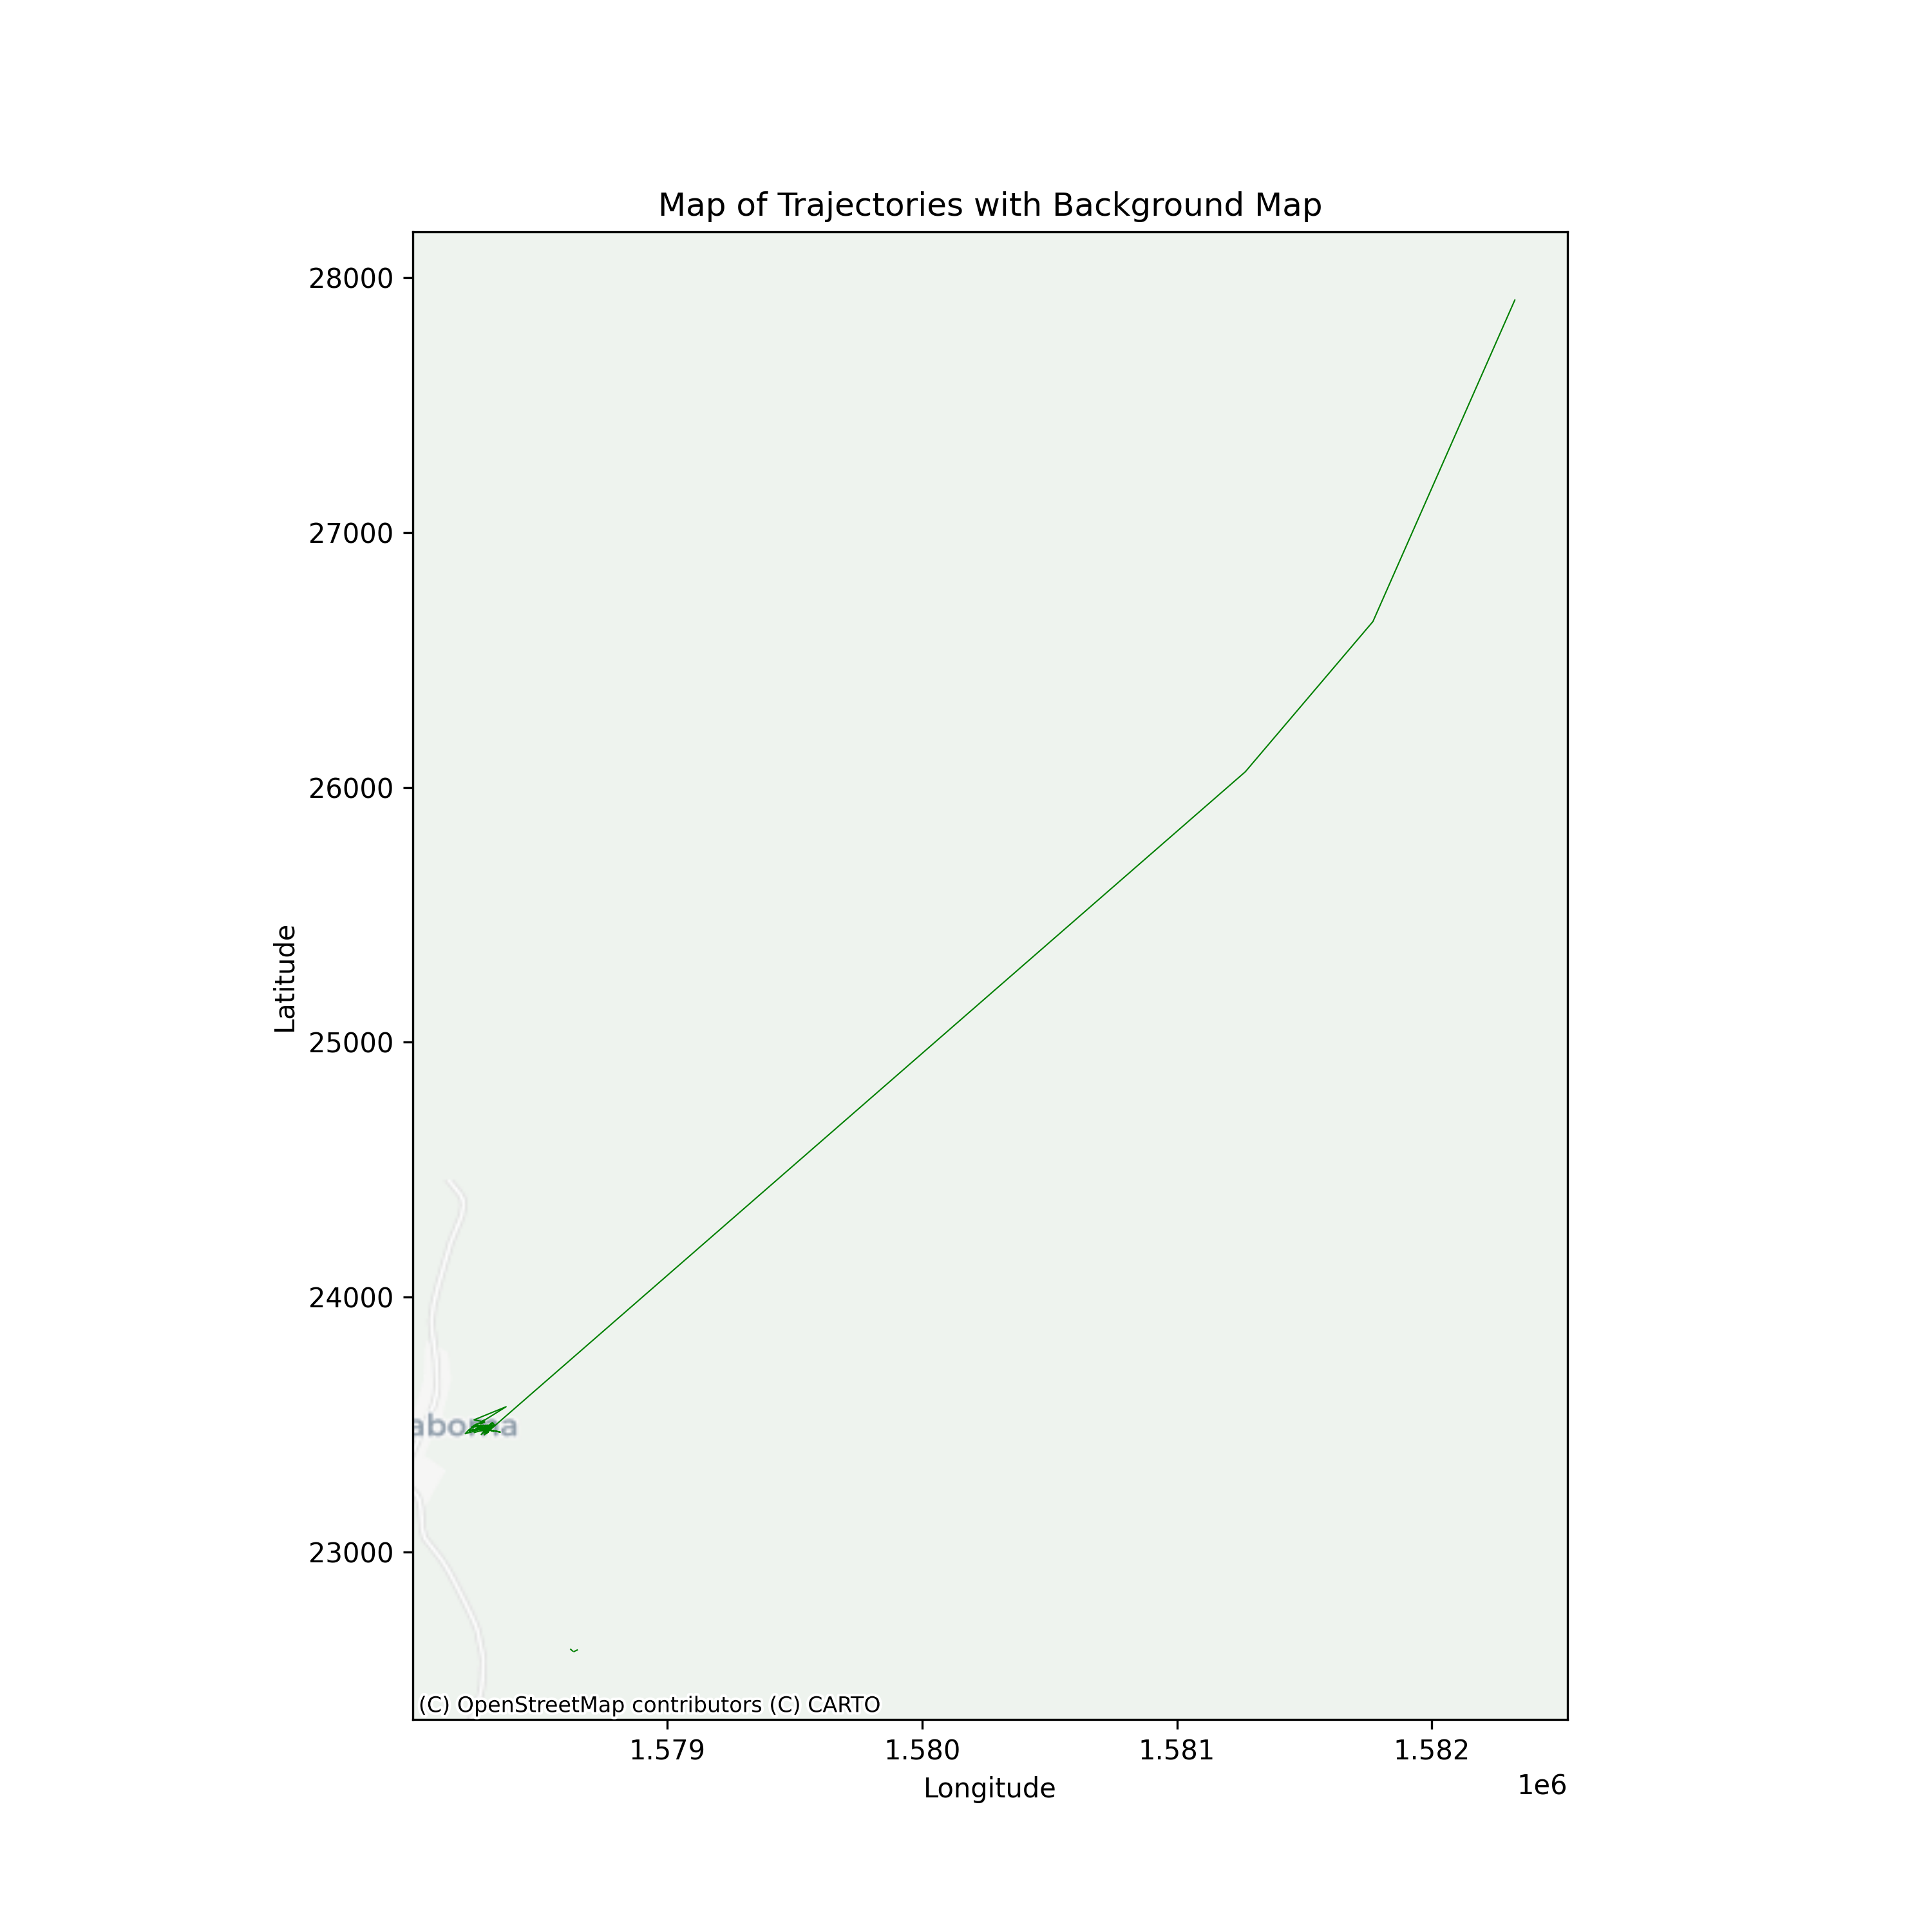
\includegraphics[width=0.5\textwidth]{img/Movebank/map_prueba_10datos.png}
    \caption{Mapa de trayectorias MoveBank, 10 filas.}
    \label{fig:movebank_10}
\end{figure}

\subparagraph{Trayectorias Taxis (10 filas)}

Este conjunto mostró trayectorias más homogéneas, con menor dispersión:

\begin{figure}[h!]
    \centering
    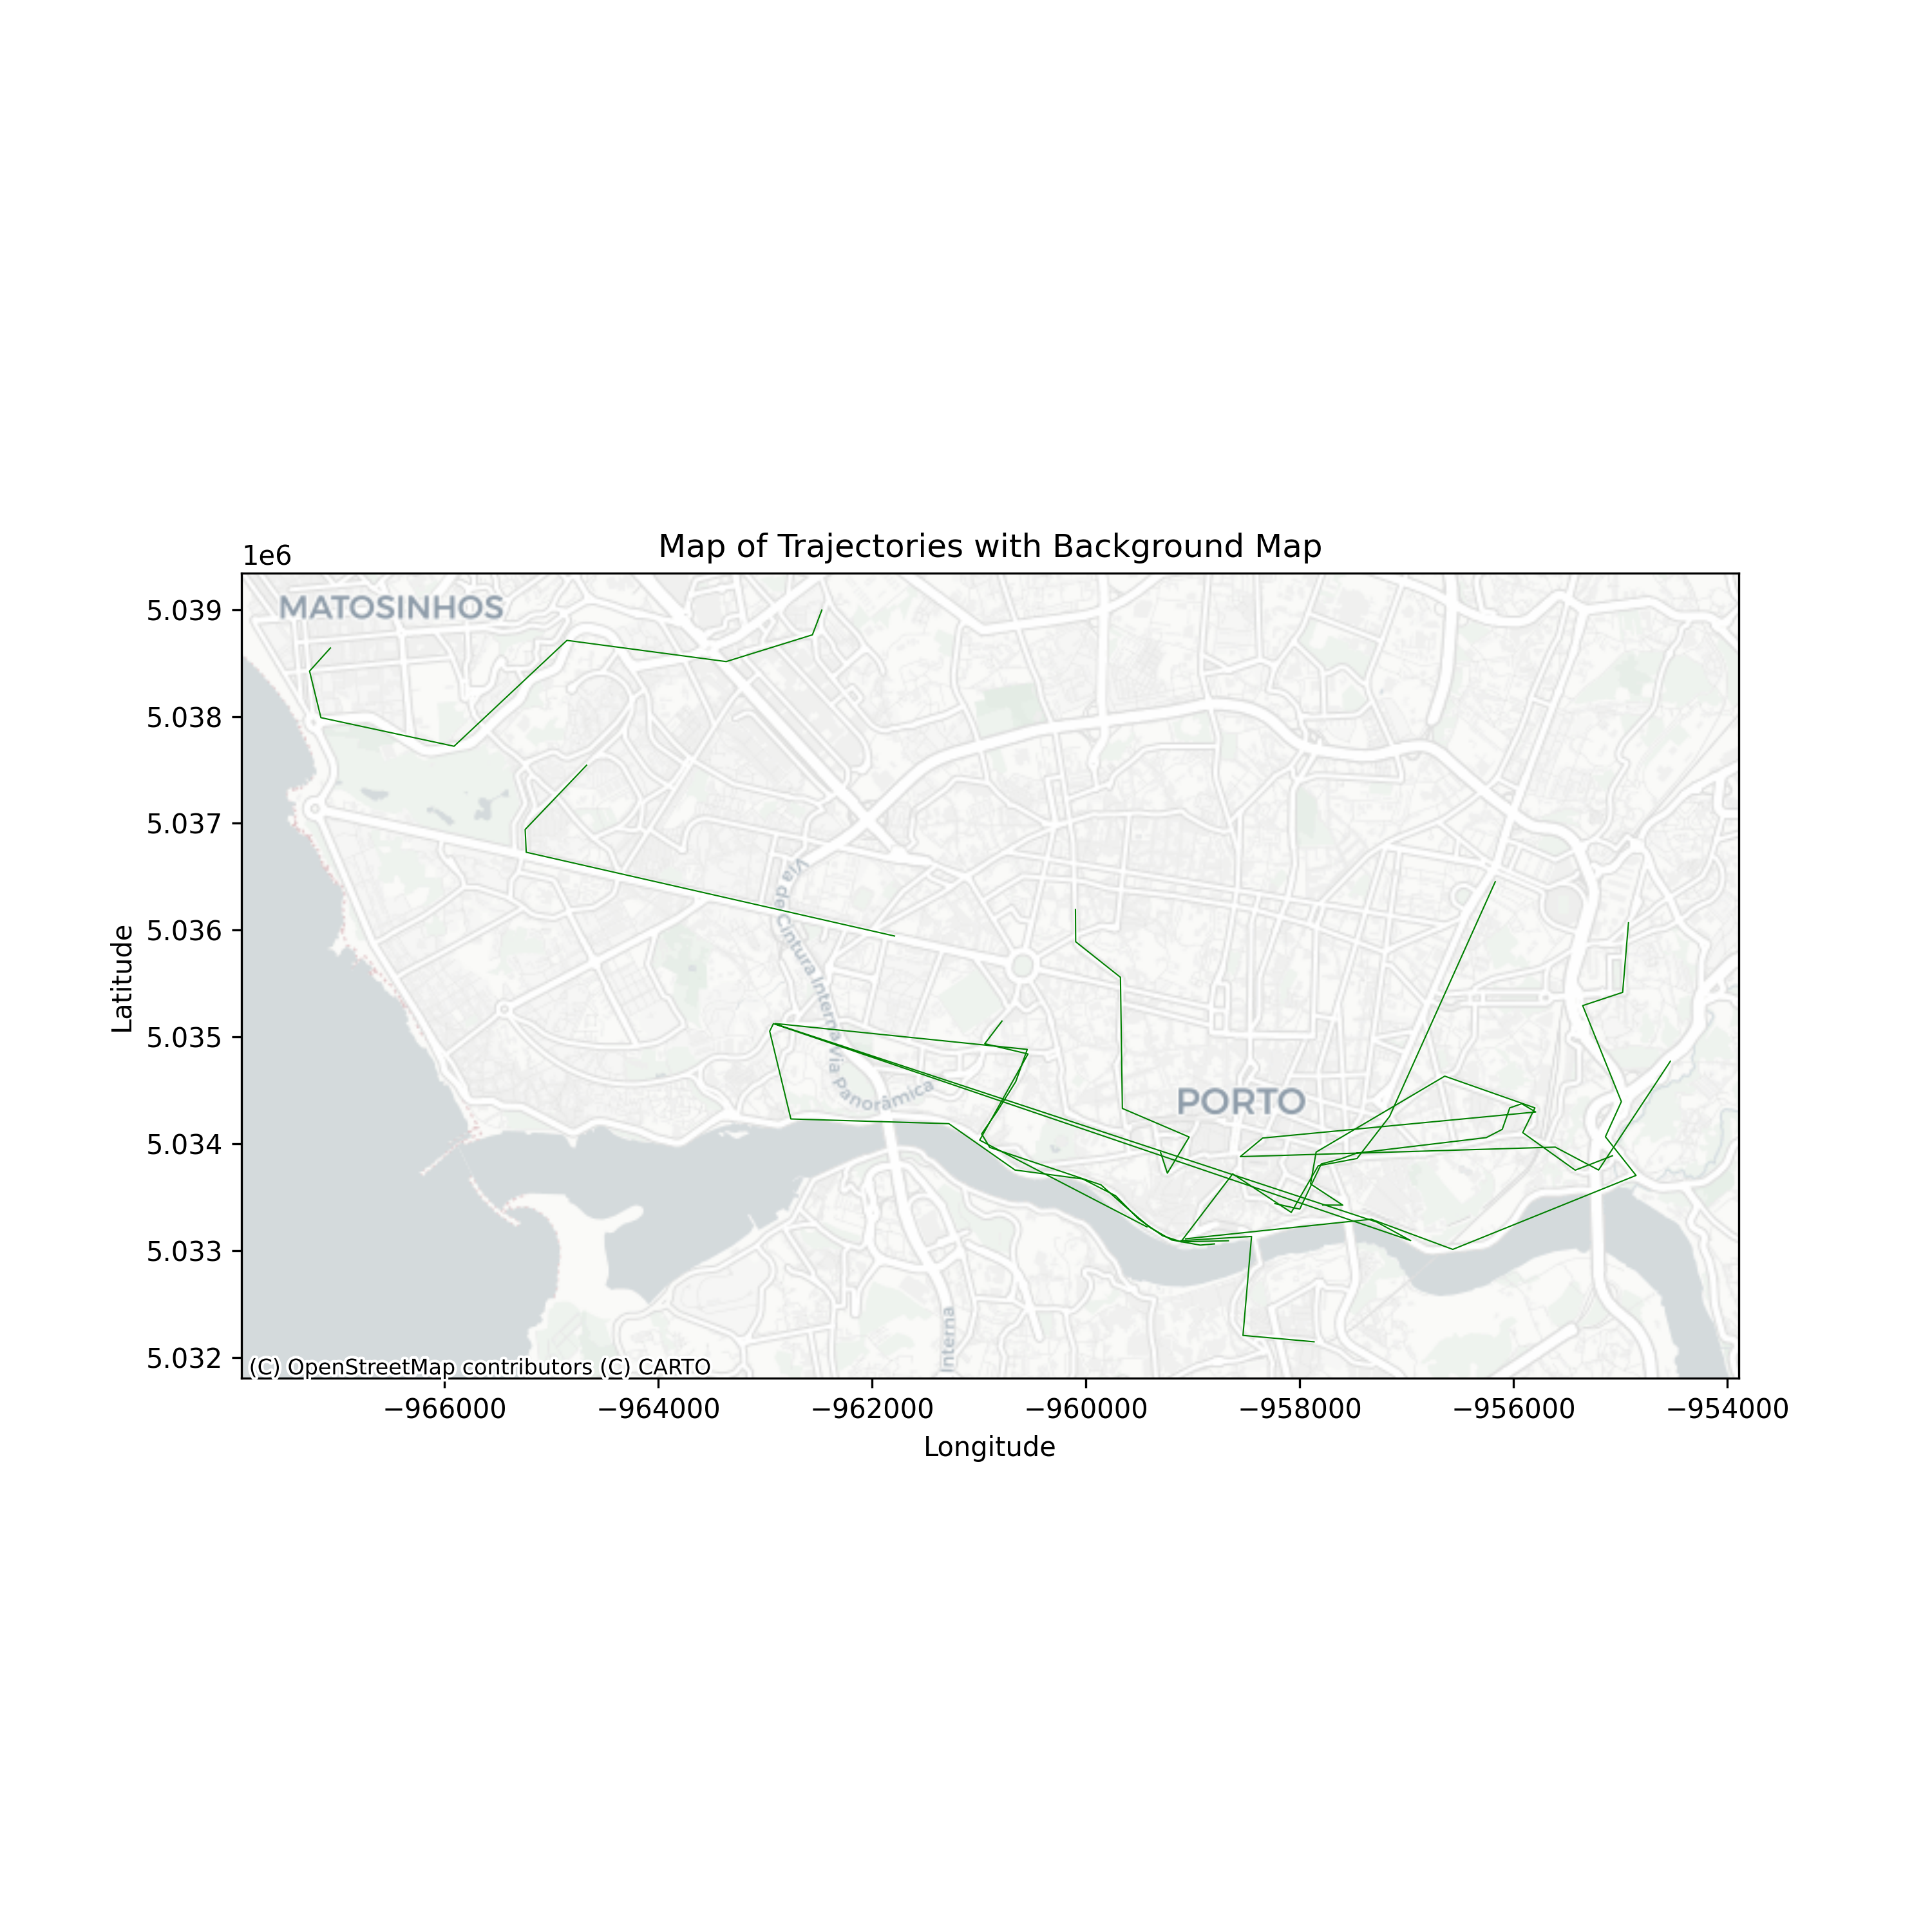
\includegraphics[width=0.5\textwidth]{img/Taxis/map_prueba_10datos.png}
    \caption{Mapa de trayectorias Taxis, 10 filas.}
    \label{fig:taxis_10}
\end{figure}

\begin{itemize}
    \item \textbf{OPTICS y DBSCAN:} Produjeron rutas consistentes.
    
	\begin{figure}[h!]
    		\centering
    		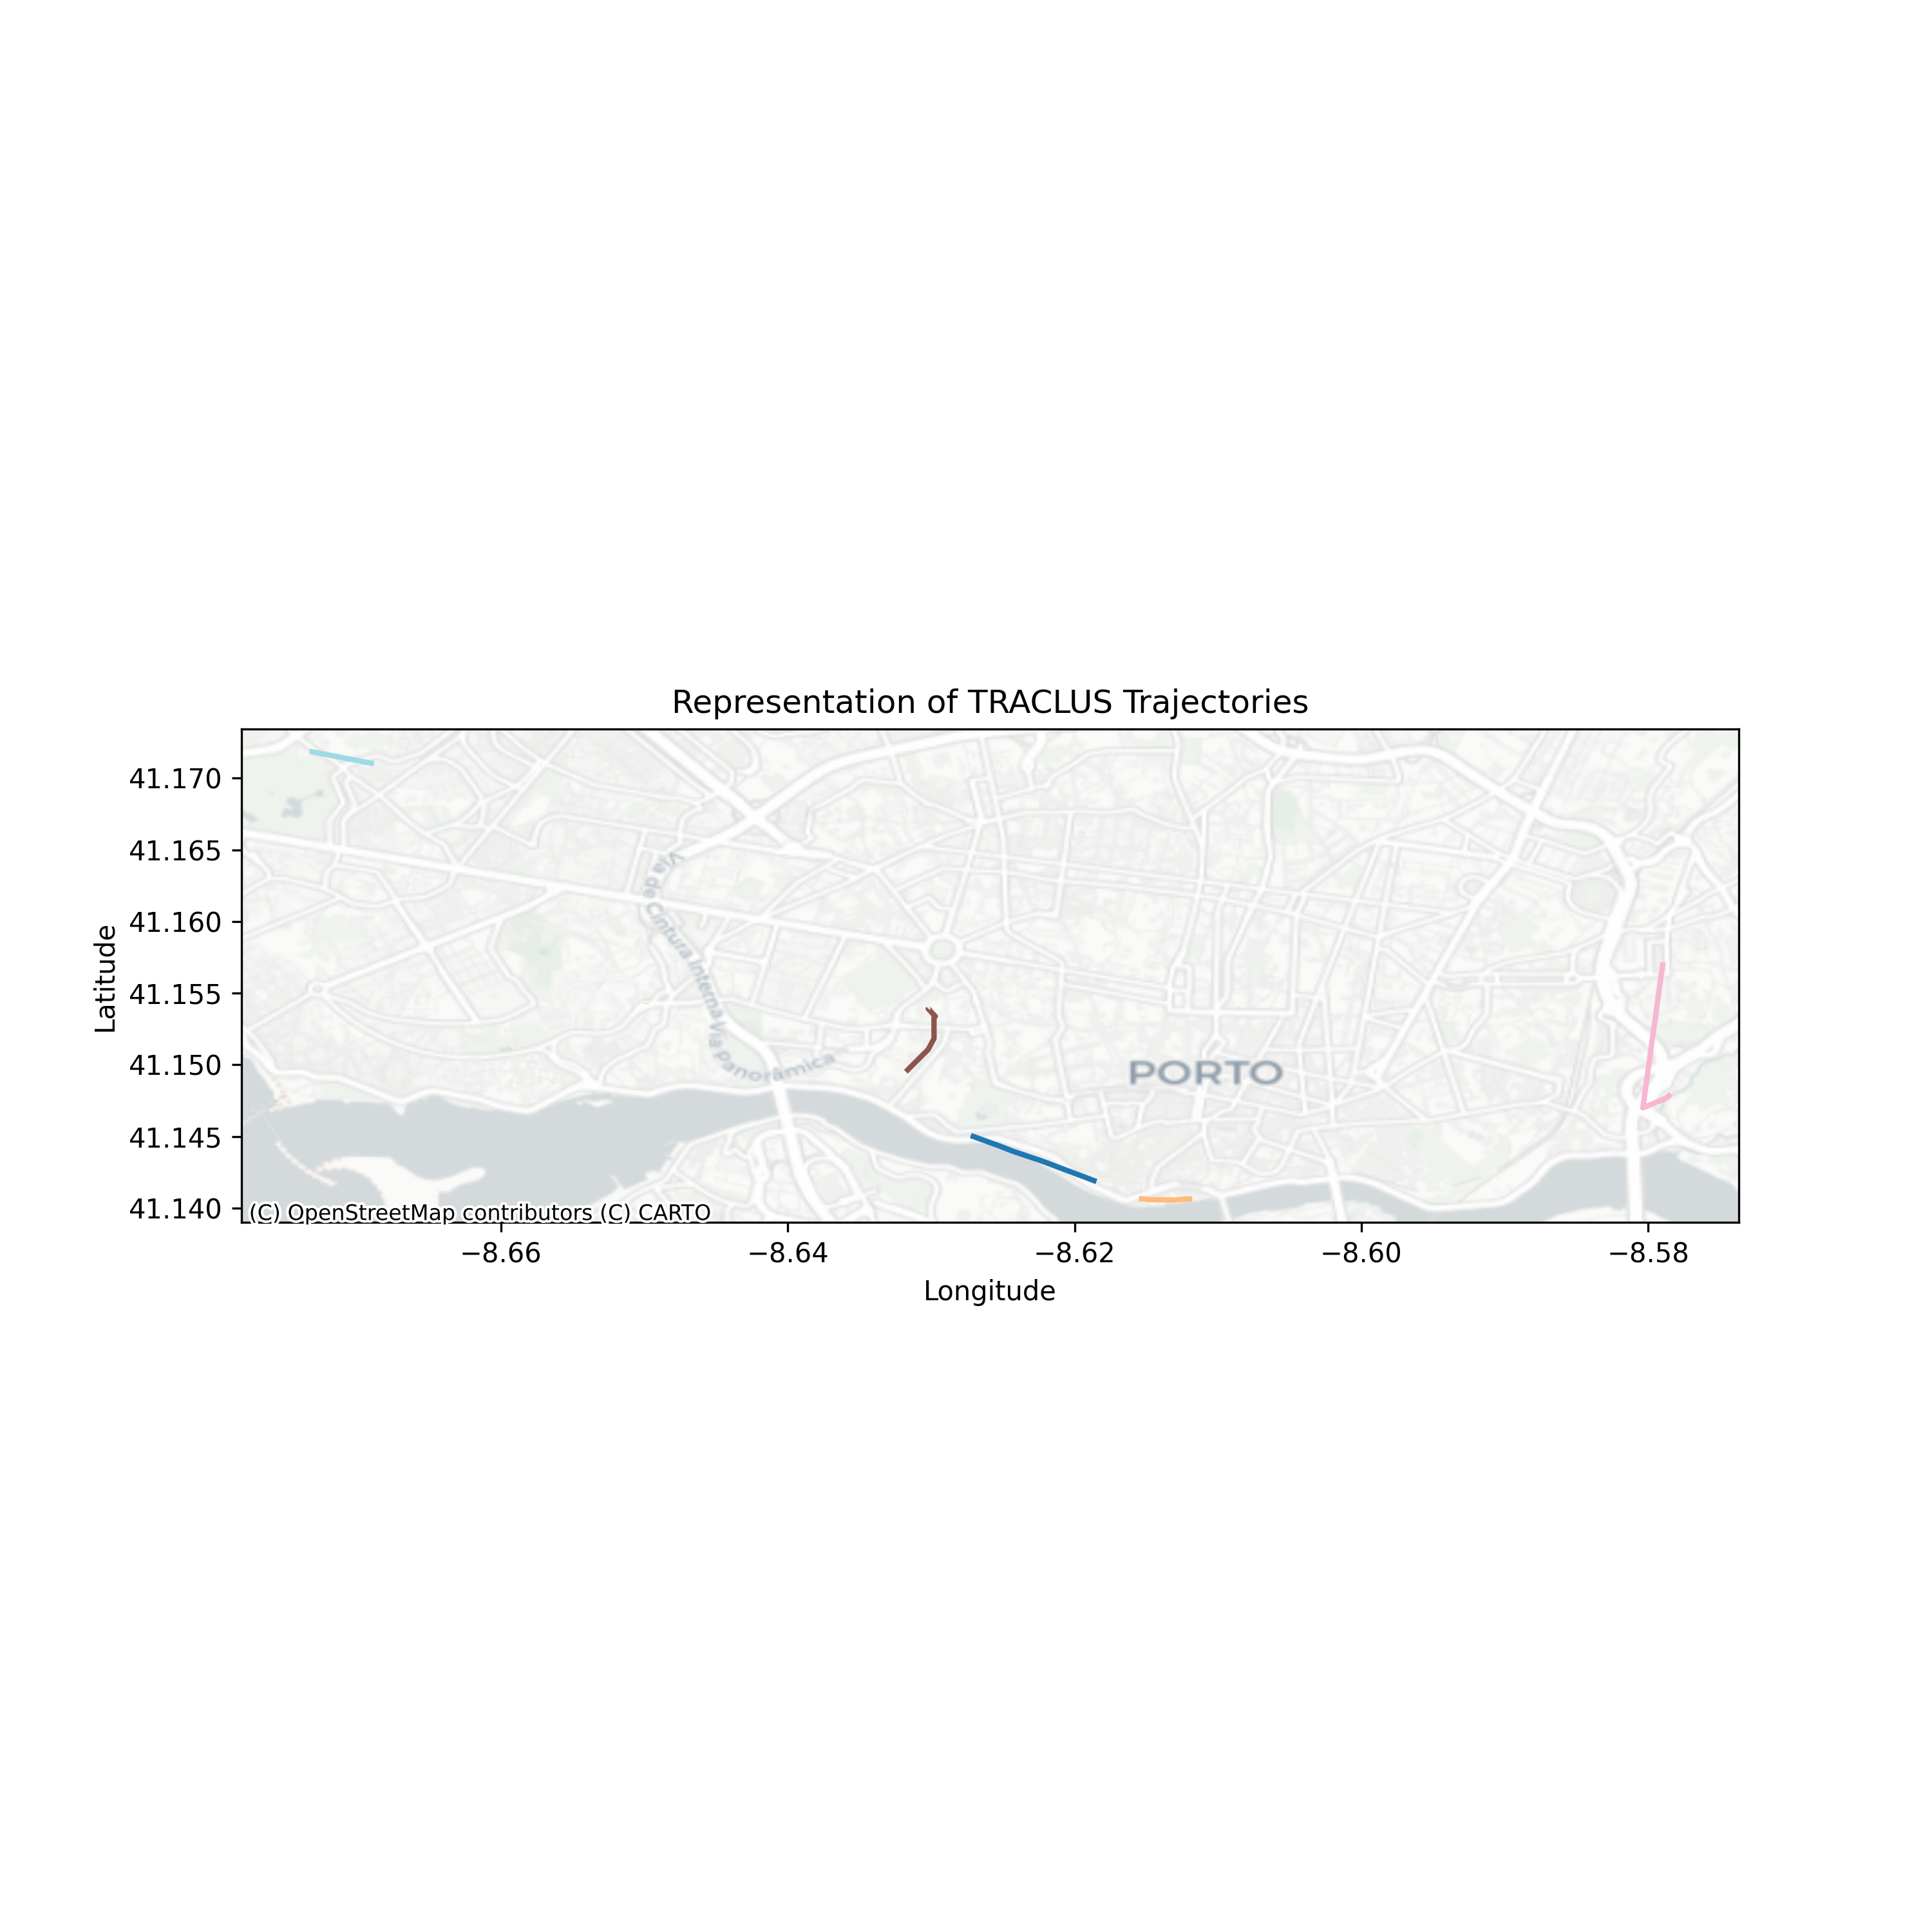
\includegraphics[width=0.5\textwidth]{img/Taxis/map_optics_10datos.png}
    		\caption{Mapa trayectorias resultantes OPTICS y DBSCAN, 10 filas.}
    		\label{fig:taxis_10}
	\end{figure}    
    
    \item \textbf{HDBSCAN:} Generó tres rutas principales, siendo una de ellas significativamente más extensa y errática.
    
    \begin{figure}[h!]
    		\centering
    		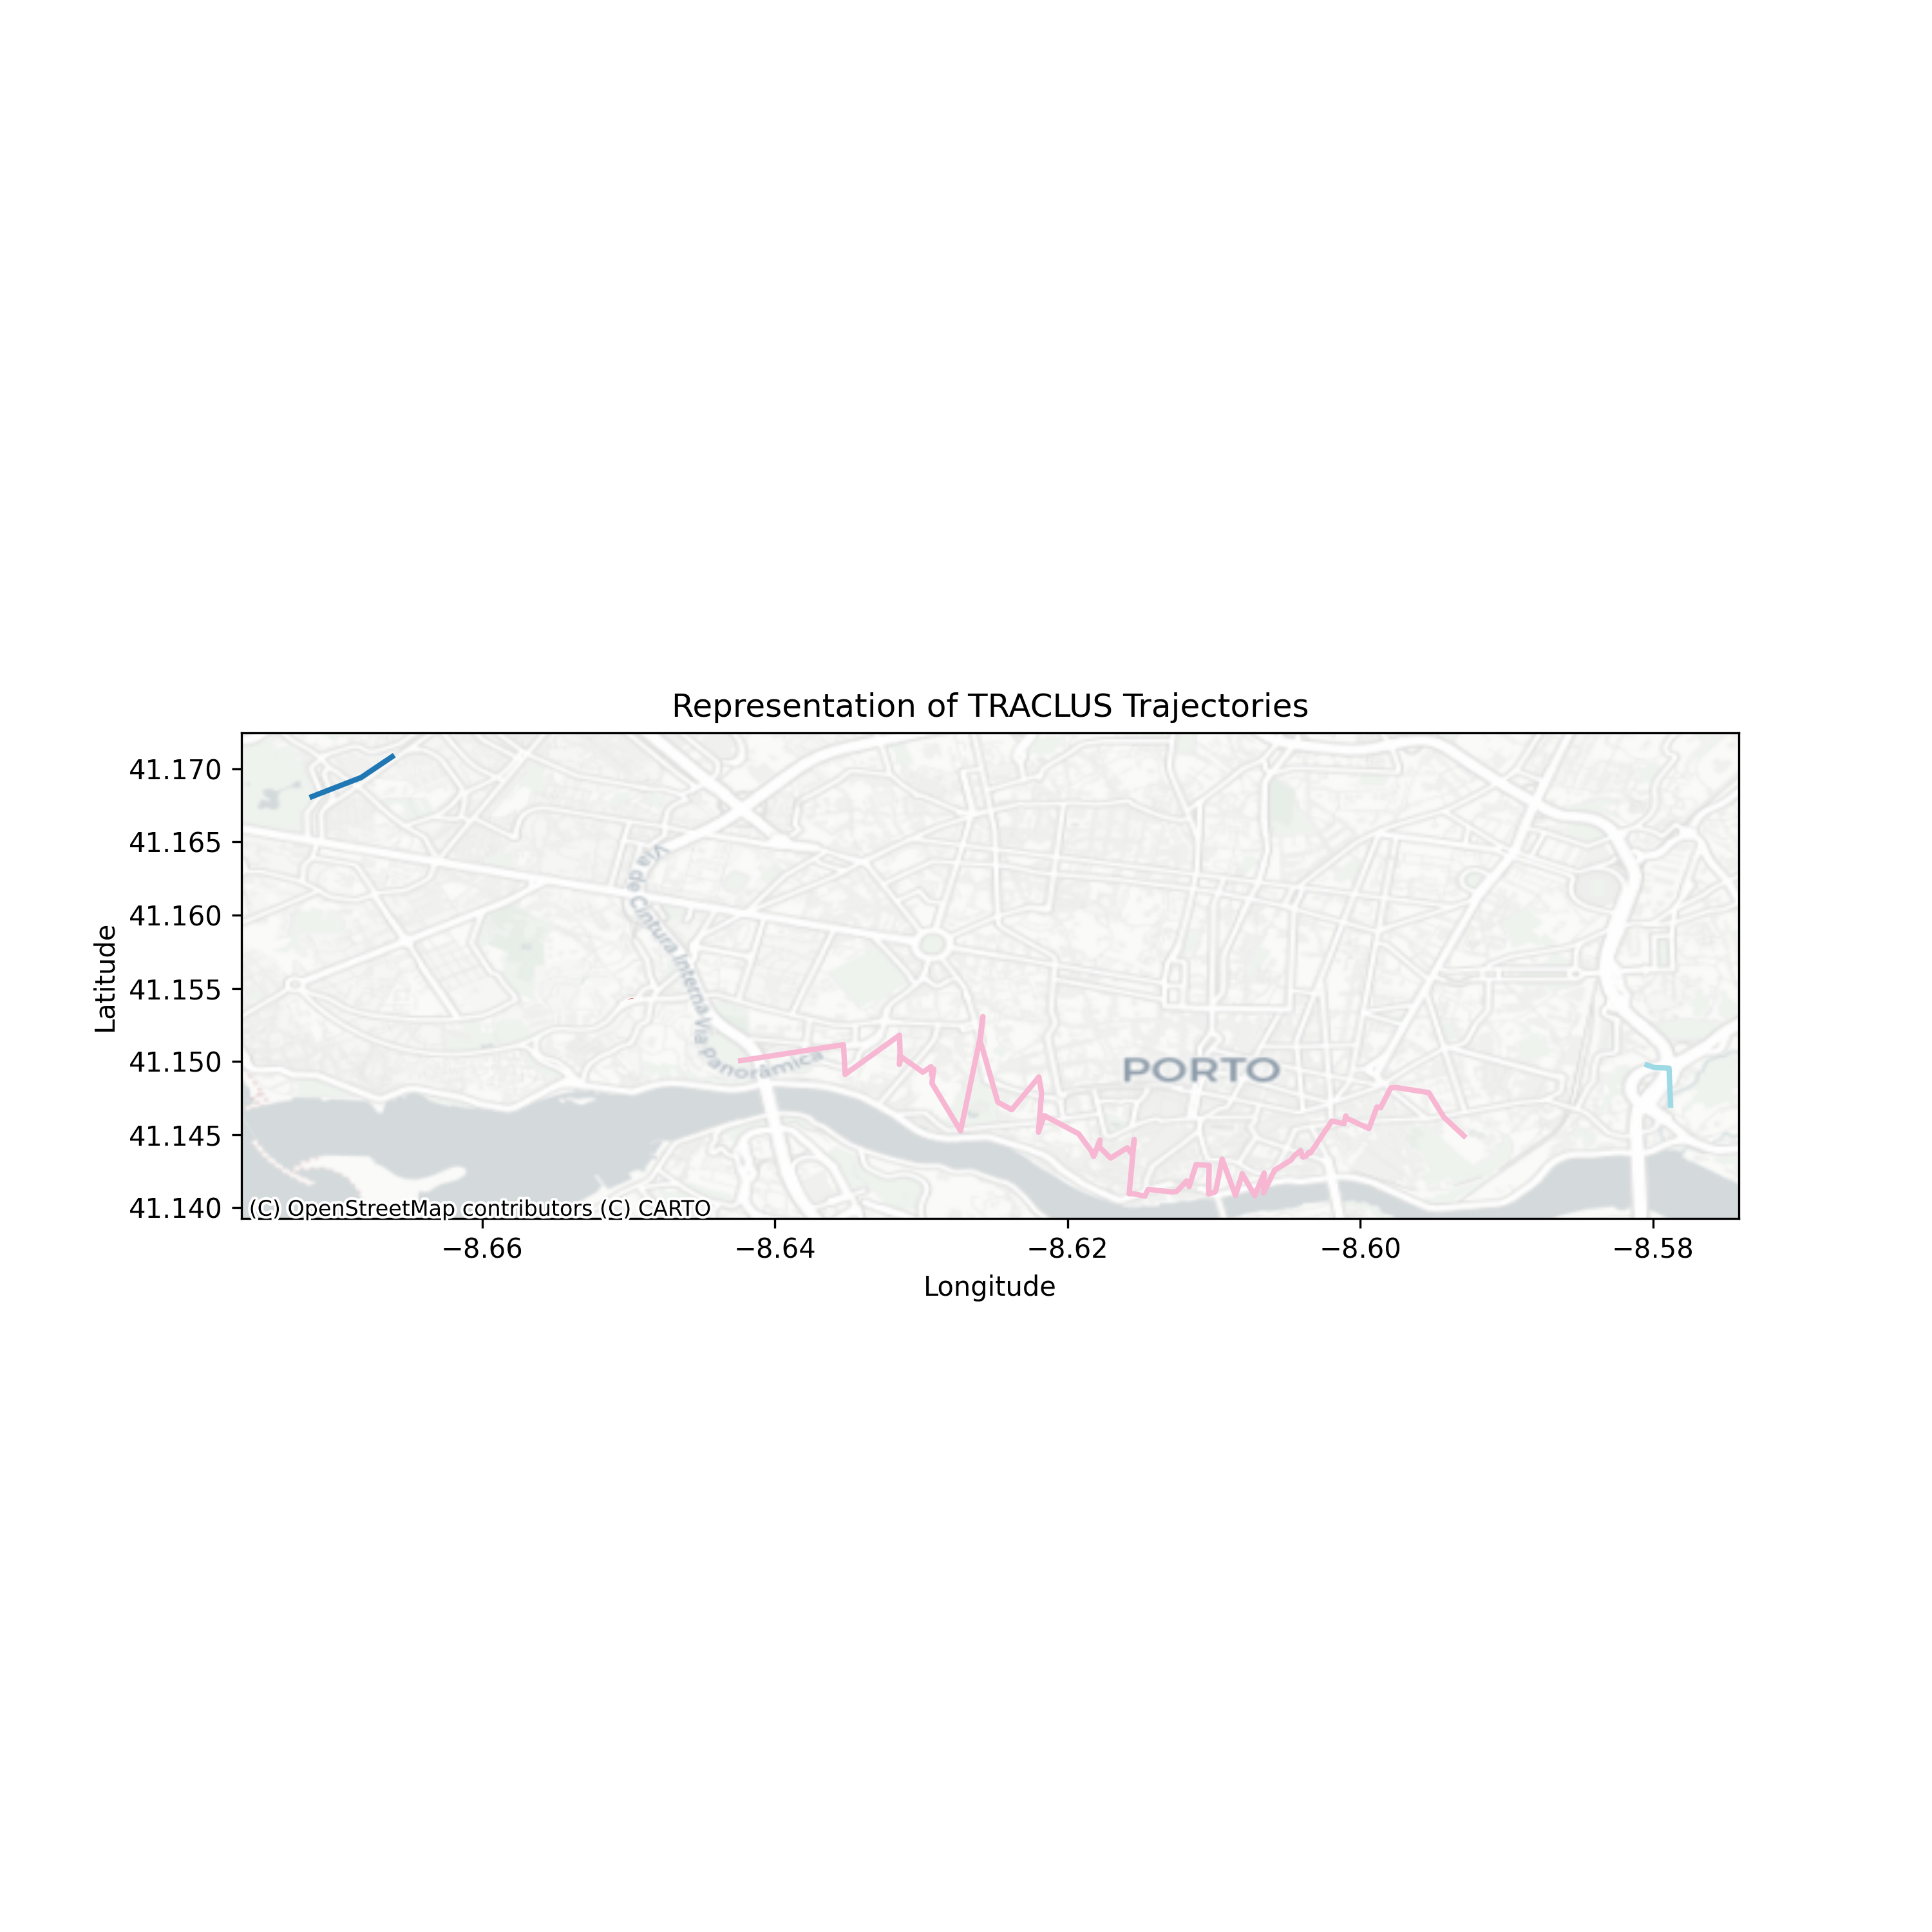
\includegraphics[width=0.5\textwidth]{img/Taxis/map_hdbscan_10datos.png}
    		\caption{Mapa trayectorias resultantes HDBSCAN, 10 filas.}
    		\label{fig:taxis_10}
	\end{figure}  
    
    \item \textbf{Agglomerative y Spectral Clustering:} Igual que los anteriores algoritmos representaron bien las zomas mas concurrentes pero su resultados restaron más erráticos debido al número de clusters predefinido.
    
    \begin{figure}[h!]
    		\centering
    		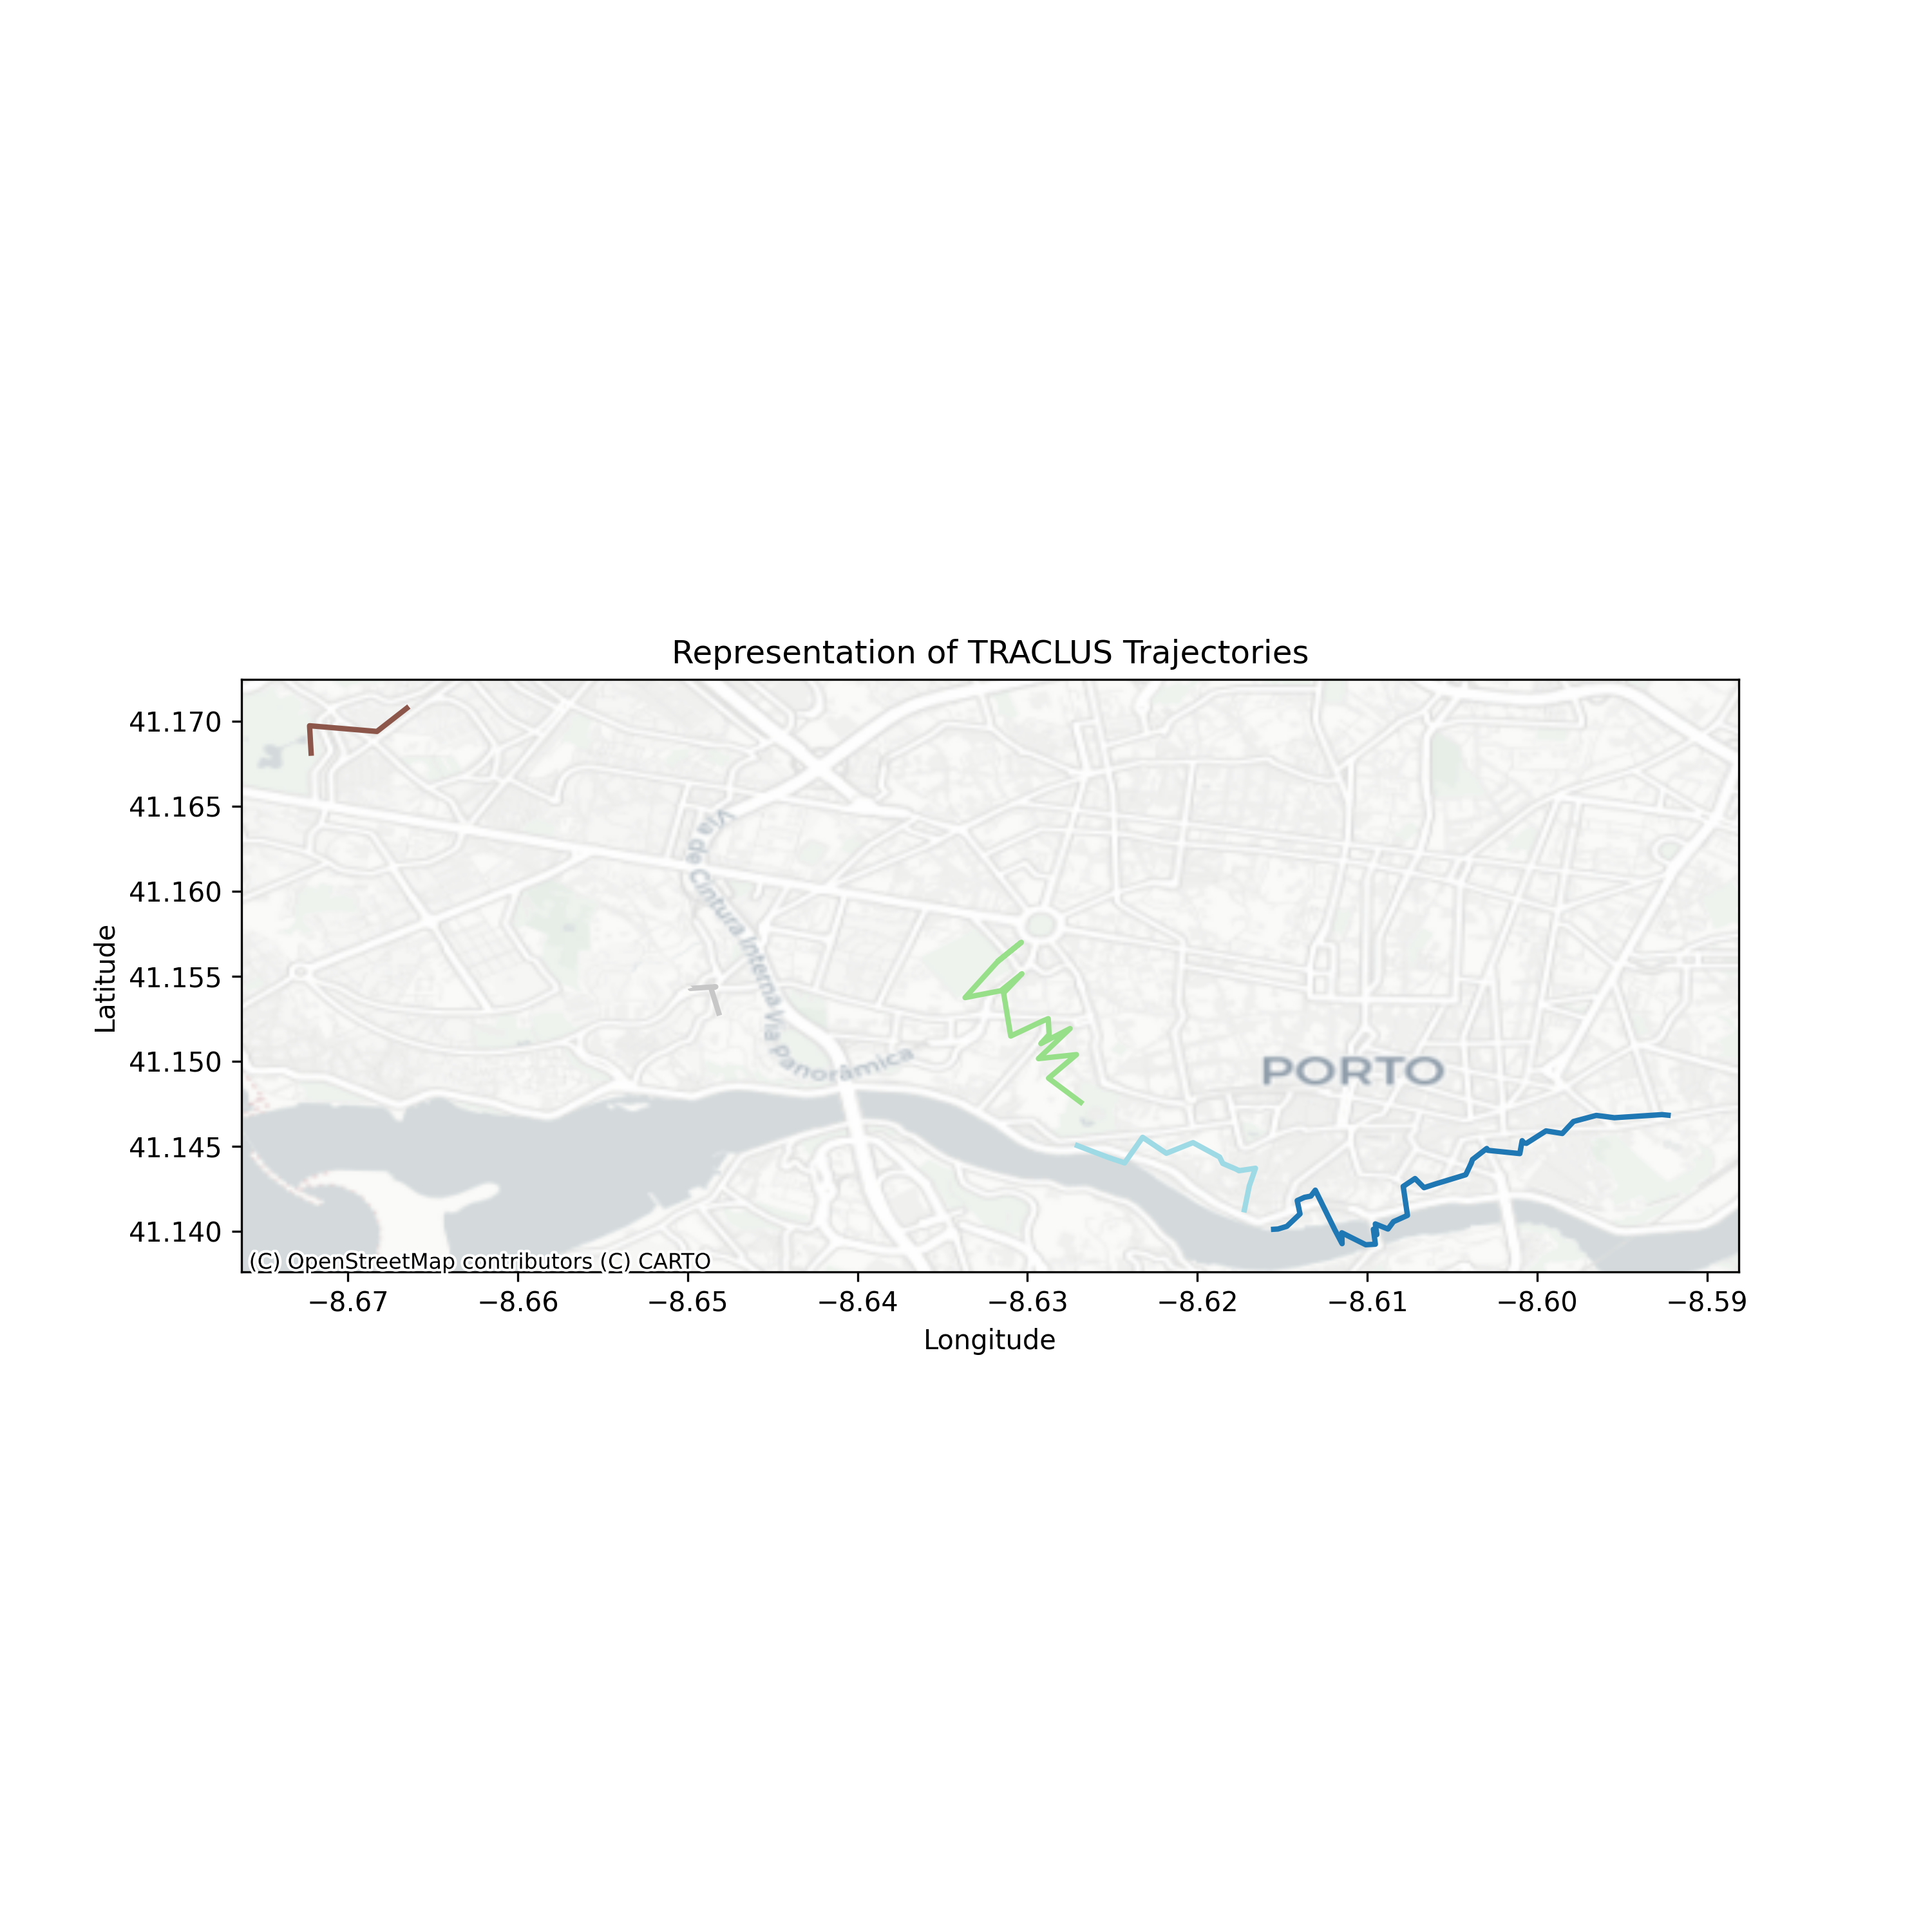
\includegraphics[width=0.5\textwidth]{img/Taxis/map_aggl_10datos.png}
    		\caption{Mapa trayectorias resultantes Agglomerative, 10 filas.}
    		\label{fig:taxis_10}
	\end{figure}  
	
	\begin{figure}[h!]
    		\centering
    		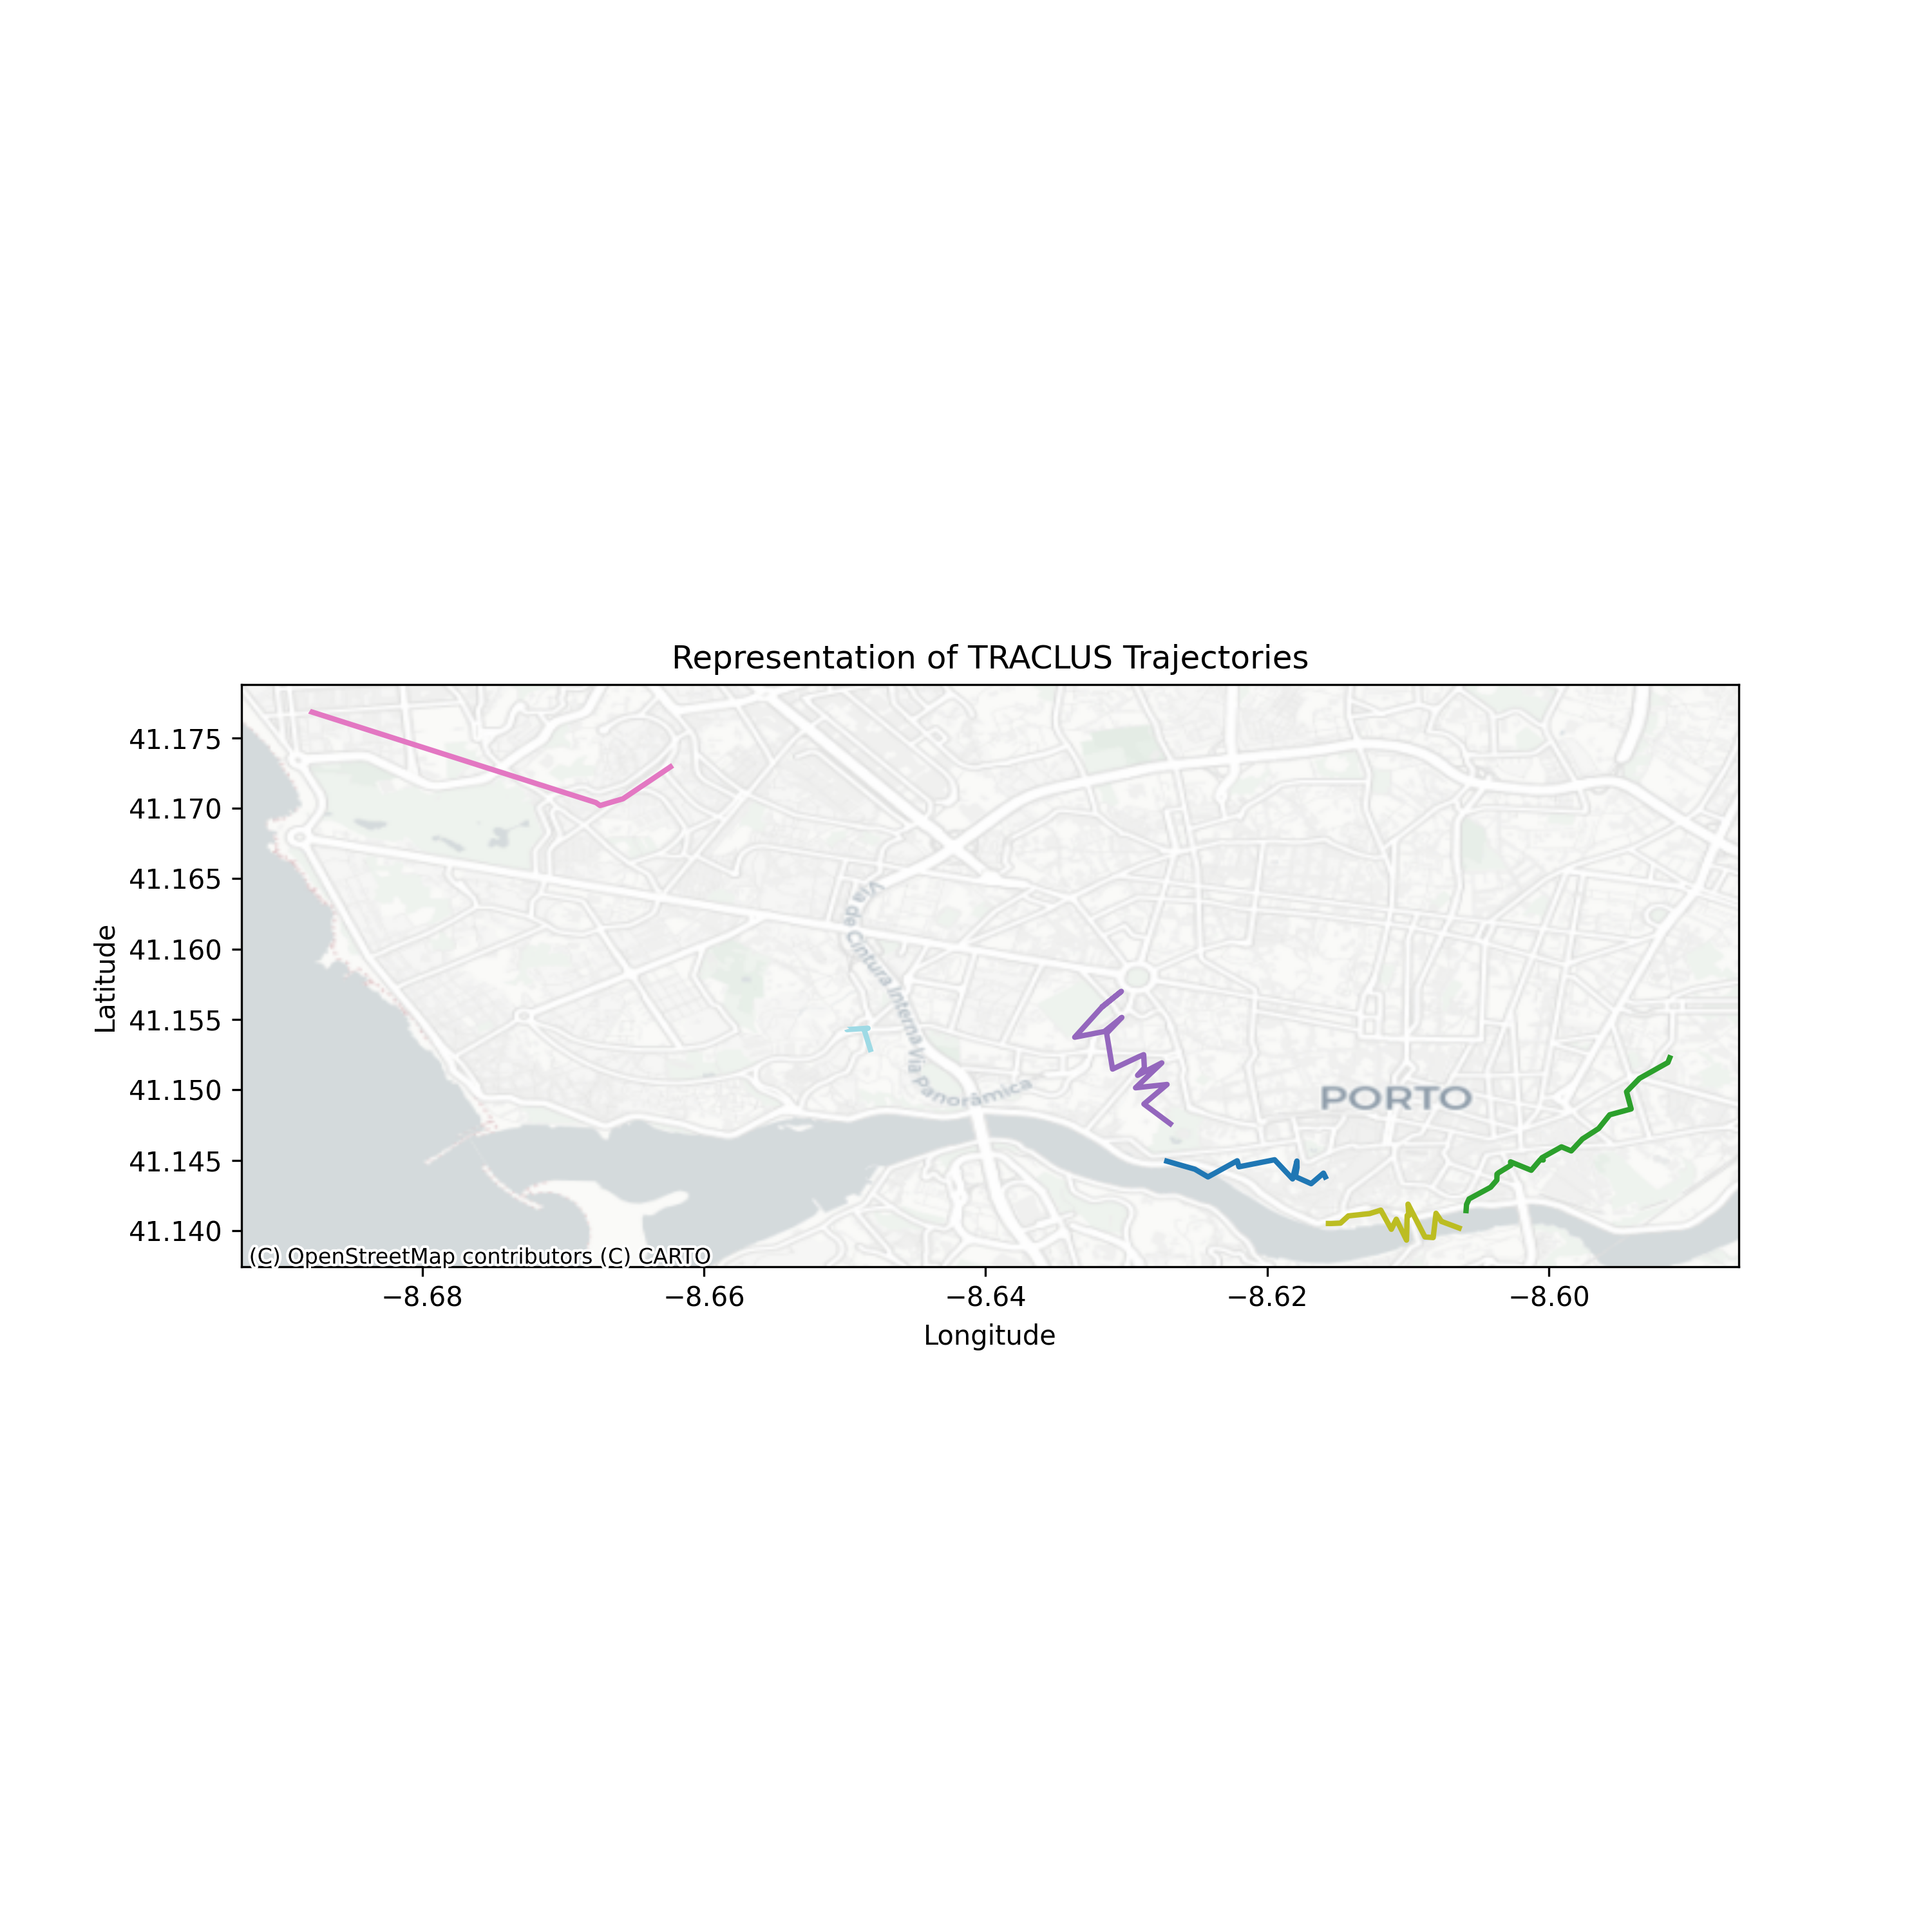
\includegraphics[width=0.5\textwidth]{img/Taxis/map_spect_10datos.png}
    		\caption{Mapa trayectorias resultantes Spectral, 10 filas.}
    		\label{fig:taxis_10}
	\end{figure}  
\end{itemize}

Estas pruebas iniciales revelaron diferencias significativas en el comportamiento de los algoritmos bajo diferentes configuraciones y conjuntos de datos, como el nuemor de culters que se generaron en todos los conjuntos, cuatro en HDBSCAN y siete en el resto. Ademas consumió una cantidad de tiempo considerable lo que predijo lo extenso que podría ser comprobar y analizar resultados de diferentes configuraciones en diferentes conjuntos de datos.




\section{Testing}

Para que un código sea verdaderamente funcional, seguro y mantenible, debe someterse a pruebas exhaustivas. Durante el desarrollo del proyecto, se implementaron varios tipos de pruebas para evaluar el rendimiento y la calidad del código, así como para ampliar el conocimiento en el campo del testing.

\subsection{Análisis de código estático}

El análisis de código estático es una técnica utilizada para identificar posibles errores en el código fuente sin necesidad de ejecutarlo. Este método es particularmente útil para evitar fallos humanos como bucles infinitos, errores de formato o problemas de nomenclatura.

Se evaluaron varias herramientas de análisis estático teniendo en cuenta las siguientes limitaciones:
\begin{itemize}
    \item Debían ser compatibles con Python y CSS, los lenguajes utilizados en el proyecto.
    \item No debían implicar costos adicionales.
    \item Era deseable la integración directa con GitHub para facilitar el flujo de trabajo.
\end{itemize}

Con estas características, se seleccionaron dos herramientas principales: \textbf{SonarQube} y \textbf{Code Climate}. De estas, \textbf{SonarQube} fue la más utilizada, ya que ofrecía soporte para analizar IPython Notebooks, un formato clave en los experimentos realizados durante el proyecto. Aunque los notebooks no formaban parte directa de la aplicación web, su análisis fue crucial para garantizar la calidad de los experimentos previos.

Lo ideal en este tipo de análisis es aplicarlo de manera continua durante las diversas fases del proyecto, ya que esto reduce significativamente la carga de trabajo y mejora la calidad del código a medida que se desarrolla. Sin embargo, en este proyecto, el análisis estático se realizó al final, lo que no fue óptimo pero permitió identificar una serie de problemas, entre ellos:

\begin{itemize}
    \item \textbf{Mejoras en nomenclatura:} Se ajustaron nombres de variables para facilitar su comprensión y evitar confusiones con otros datos.
    
\begin{figure}[h!]
    \centering
    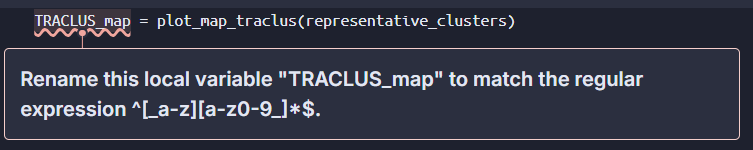
\includegraphics[width=0.5\textwidth]{img/sonarq_regularexp.png}
    \caption{Error nomenclatura.}
    \label{fig:trayectorias_Spectral}
\end{figure}    
    
    \item \textbf{Variables no utilizadas:} Se detectaron y eliminaron variables que ya no eran relevantes, ya fuera por errores en su definición o por haber quedado obsoletas durante el desarrollo.
    
\begin{figure}[h!]
    \centering
    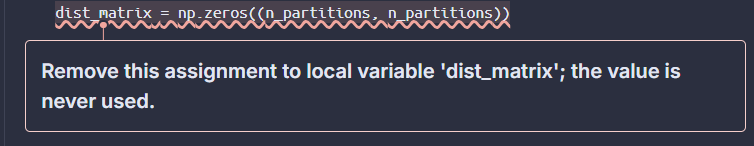
\includegraphics[width=0.5\textwidth]{img/sonarq_codigo_sobrante.png}
    \caption{Código innecesario.}
    \label{fig:trayectorias_Spectral}
\end{figure}

\begin{figure}[h!]
    \centering
    
\includegraphics[width=0.5\textwidth]{img/sonarq_unused.png}
    \caption{Variable sin usar necesaria.}
    \label{fig:trayectorias_Spectral}
\end{figure}    
    
    \item \textbf{Importaciones innecesarias:} Se eliminaron módulos y librerías no utilizadas, lo que ayudó a reducir la carga del programa y mejorar su legibilidad.
    
\begin{figure}[h!]
    \centering
    
\includegraphics[width=0.5\textwidth]{img/sonarq_imports.png}
    \caption{Importación excesiva.}
    \label{fig:trayectorias_Spectral}
\end{figure}
   
    \item \textbf{Complejidad en funciones:} Se identificaron funciones cuya complejidad excedía los límites recomendados. Aunque algunas de estas funciones no pudieron simplificarse debido a las características del algoritmo, el análisis ayudó a priorizar futuras mejoras.
    
\begin{figure}[h!]
    \centering
    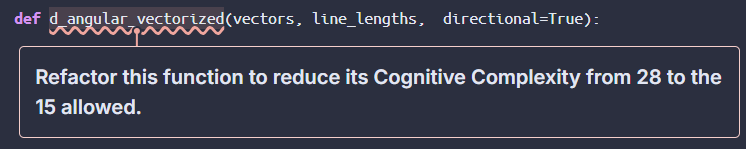
\includegraphics[width=0.5\textwidth]{img/sonarq_complex.png}
    \caption{Complejidad grande.}
    \label{fig:trayectorias_Spectral}
\end{figure}

\end{itemize}

Aunque este tipo de análisis no corrige directamente errores en la funcionalidad del algoritmo, resulta muy útil para evitar problemas menores, mejorar la mantenibilidad del código y garantizar un nivel básico de seguridad.

\subsection{Pruebas unitarias y su implementación}

Las pruebas unitarias son fundamentales para garantizar la funcionalidad de cada componente del código y asegurar que los resultados generados sean consistentes y correctos. Durante el desarrollo de la aplicación, se planteó inicialmente realizar pruebas unitarias utilizando \texttt{pytest} que evaluaran el comportamiento de cada botón y función de la aplicación mientras esta se ejecutaba. El objetivo era cubrir todo el flujo de la web en tiempo real, desde la interacción del usuario con los botones hasta la ejecución de los \texttt{callbacks} de Dash.

Sin embargo, esta aproximación presentó múltiples problemas. Dash, como framework basado en componentes interactivos, no es directamente compatible con las herramientas de testing tradicionales. Intentar realizar pruebas unitarias mientras la aplicación se encontraba en ejecución resultó inviable, ya que las pruebas no se ejecutaban correctamente, y la interacción con los componentes de la interfaz gráfica no podía ser simulada adecuadamente. Como resultado, las pruebas terminaban siendo llamadas directas a las funciones asociadas a los botones, sin representar el comportamiento real del flujo de la aplicación ni garantizar que los \texttt{callbacks} funcionaran en contexto.

Ante esta limitación, se decidió cambiar el enfoque hacia pruebas más efectivas y relevantes. La nueva estrategia consistió en lo siguiente:

\begin{itemize}
    \item \textbf{Pruebas de funciones críticas:} Se probaron de manera individual las funciones más importantes de los modelos, como la implementación del algoritmo TRACLUS y su integración con diferentes algoritmos de clustering. Estas pruebas se realizaron utilizando conjuntos de datos generados de manera aleatoria para garantizar que el comportamiento del código fuese robusto ante diferentes escenarios.
    \item \textbf{Representación de mapas:} Se verificó que las funciones encargadas de generar mapas, tanto de segmentos como de clústeres, produjeran respuestas correctas. 
\end{itemize}